% MFTL2 — user and developer manual.
% Build: make -C doc   (see doc/README.md). The listings are included from ../examples/, which
% the library's test suite compiles and runs, so every listing is a working program.
\documentclass[11pt,a4paper]{report}

\usepackage[T1]{fontenc}
\usepackage[utf8]{inputenc}
\usepackage{lmodern}
\usepackage[margin=2.5cm]{geometry}
\usepackage{microtype}
\usepackage{amsmath,amssymb}
\usepackage{booktabs,tabularx,longtable,multirow}
\usepackage{enumitem}
\usepackage{xcolor}
\usepackage{listings}
\usepackage{tikz}
\usetikzlibrary{arrows.meta,calc,decorations.markings,positioning,patterns,shapes.geometric}
\usepackage{caption}
\usepackage[colorlinks,linkcolor=black,citecolor=black,urlcolor=blue!50!black]{hyperref}

\setlength{\parindent}{0pt}
\setlength{\parskip}{0.6ex plus 0.2ex}
\setlist{itemsep=0.2ex,topsep=0.4ex}
\setlength{\emergencystretch}{3em}
% identifiers may break after an underscore
\renewcommand{\_}{\textunderscore\allowbreak}

\definecolor{dkgreen}{rgb}{0,0.45,0}
\definecolor{gray}{rgb}{0.5,0.5,0.5}
\definecolor{mauve}{rgb}{0.5,0,0.6}
\lstset{language=C, basicstyle=\footnotesize\ttfamily, numbers=left, numberstyle=\tiny\color{gray},
  numbersep=5pt, frame=single, rulecolor=\color{black!40}, tabsize=2, breaklines=true,
  showstringspaces=false, keywordstyle=\color{blue!70!black}\bfseries,
  commentstyle=\color{dkgreen}\itshape, stringstyle=\color{mauve}, columns=fullflexible,
  keepspaces=true, captionpos=b,
  morekeywords={bool,size_t,MFTL_Object,MFTL_Ensemble,MFTL_Domain,MFTL_Vertex,MFTL_Triangle,MFTL_HalfEdge}}

% MFTL2 names
\newcommand{\mftl}{\textsf{MFTL2}}
\newcommand{\mftlone}{\textsf{MFTL1}}
\newcommand{\multi}{\textsf{multiflow}}
\newcommand{\fn}[1]{\texttt{#1}}
\newcommand{\vect}[1]{\boldsymbol{#1}}
\newcommand{\ie}{i.e.\ }
\newcommand{\eg}{e.g.\ }

\title{\textbf{MFTL2}\\[1ex] \large The MultiFlow Triangle Library, version 2\\ User and developer manual}
\author{}
\date{Describes MFTL2 after Stage 16 (generalized periodic and open surfaces)\\ and the Stage-17 source layout}

\begin{document}
\maketitle
\tableofcontents

\chapter{Introduction}
\label{ch:intro}

\section{What is MFTL2?}

\mftl{} is a C99 library for triangulated surfaces that are distributed over the ranks of an MPI
program. It stores the surfaces, moves them between ranks as they move through space, computes
their geometry (normals, curvature, areas, volumes, centres, moments of inertia), answers
point and intersection queries, and keeps their mesh quality under control by remeshing. It is
the surface engine of the front-tracking and immersed-boundary methods of the \multi{} flow
solver, where a surface is advected by the flow, carries forces and scalars, and is
remeshed every few time steps.

The surfaces it handles are
\begin{itemize}
  \item \textbf{closed} surfaces (bubbles, drops, particles) in a bounded or periodic box;
  \item \textbf{periodic} surfaces: a closed body that crosses a periodic boundary (a
    \emph{seam}), and surfaces that \emph{wrap} a periodic direction --- a ribbon that spans the
    box along $x$, a film that spans $x$ and $y$, a surface that wraps all three directions;
  \item \textbf{open} surfaces with a physical boundary (a membrane pinned on a ring, a cap on a
    wall orifice, a patch), declared as open by the application.
\end{itemize}
Every combination is supported: an open surface may cross periodic seams, a wrapping film may
be cut by many rank boundaries.

This manual describes \mftl{} as it exists after Stage~16 of its development (generalized
periodic and open surfaces) with the source layout of Stage~17. It explains the concepts
first --- the data structures, the parallel model, the invariants the library maintains ---
and then the functions that act on them. Every code listing in the manual is a complete
program from the \texttt{examples/} directory; the test suite compiles and runs them on 1, 2,
4 and 8 ranks, so they work as printed.

\section{Differences from MFTL1}
\label{sec:mftl1}

\mftl{} is a rewrite of the original MultiFlow Triangle Library (\mftlone). It keeps the
numerical conventions of \mftlone{} wherever \multi{} depends on them --- the mean-curvature
convention $2/R$, the remeshing criteria (with an explicit \mftlone{}-parity mode), the volume
recovery, the overlap quantification --- but replaces the data structures and the parallel
machinery. Table~\ref{tab:mftl1} summarises the differences. \mftlone{} identifiers appear in
this manual only in such historical comparisons.

\begin{table}[ht]
\centering\small
\begin{tabularx}{\textwidth}{@{}lXX@{}}
\toprule
 & \mftlone & \mftl \\
\midrule
Mesh storage & three hash tables (uthash) of vertices, edges and triangles & flattened arrays of vertices, triangles and half-edges per object; \texttt{khash} maps from global id to array index \\
Identity & sequential \texttt{id} & \texttt{global\_id} (unique per object across ranks) plus a rank-local array index \\
Ownership & \texttt{processor} field & \texttt{owner\_proc} and \texttt{is\_ghost}; exactly one owner per entity \\
Topology & edge records & half-edges with a twin state (LOCAL / REMOTE / BOUNDARY) \\
Decomposition & x-only 1-D ownership ranges & MPI Cartesian (or rectilinear) decomposition with a 26-neighbour graph communicator; the x-only scheme remains for load-balanced remeshing \\
Spatial search & oriented bounding-box tree & axis-aligned boxes and a linear bounding-volume hierarchy (LBVH) \\
Periodicity & not supported & periodic axes, image counters, winding classes, wrapping surfaces \\
Open surfaces & not supported & declared open bodies with tagged physical boundaries and boundary loops \\
Closed-phase quantities of general surfaces & --- & phase-boundary sets with an explicit DEFINED / UNDEFINED / UNSUPPORTED status \\
LAPACK & required & optional (paraboloid fits; a barycentric fit replaces it when absent) \\
\bottomrule
\end{tabularx}
\caption{\mftlone{} and \mftl{} compared.}
\label{tab:mftl1}
\end{table}

\section{Conventions used throughout}
\label{sec:conventions}

\begin{description}
\item[Return codes.] Functions that can fail return \texttt{MFTL\_SUCCESS} (0) or
  \texttt{MFTL\_ERROR} ($-1$). A collective function returns the same code on every rank.
\item[Collective vs.\ rank-local.] A \emph{collective} function must be called by every rank of
  the ensemble's communicator, in the same order and with the same arguments where the
  documentation says so (\eg the same query point). A \emph{rank-local} function works on the
  entities stored on the calling rank only. The documentation of every function in the headers
  states which it is.
\item[Winding.] Closed bodies are wound \emph{outward}: the triangle normal
  $(\vect{x}_1-\vect{x}_0)\times(\vect{x}_2-\vect{x}_0)$ points out of the body, and the
  enclosed volume is positive. Generators and readers canonicalise closed bodies to this
  winding.
\item[Curvature.] The stored mean curvature is $2H$, the magnitude of the discrete
  Laplace--Beltrami vector: $2/R$ on a sphere of radius $R$. The Gaussian curvature follows the
  \mftlone{} convention $2\times$(angle deficit)/(mixed area): $2/R^2$ on a sphere.
\item[Tolerances.] \texttt{MFTL\_VERYSMALL} ($10^{-12}$) and \texttt{MFTL\_VERYVERYSMALL}
  ($10^{-15}$) are fixed absolute guards against division by zero and degenerate geometry;
  \texttt{MFTL\_EPSILON} is $10^{-9}$. Decisions that depend on the scale of the mesh use
  mesh-relative tolerances inside the modules that take them. The overlap module uses the
  \mftlone{} slack \texttt{MFTL\_REL\_TOLERANCE} ($5\times10^{-7}$).
\item[Rank independence.] Integrals, loops, phase-set statuses and remeshing decisions that are
  documented as collective produce the same result on every rank. Integrals are reductions and
  may differ in the last bits between runs on different rank counts; the tests compare them with
  tolerances where that is the case.
\end{description}

\section{Glossary}
\label{sec:glossary}

\begin{description}[style=nextline,leftmargin=2.5em]
\item[object (body)] One surface, possibly with several connected components:
  \texttt{MFTL\_Object}. Identified by its object id (\texttt{global\_id} of the object).
\item[ensemble] The library handle \texttt{MFTL\_Ensemble}: one domain and the objects living
  in it. Every rank holds the same list of objects in the same order.
\item[domain] The global box, its periodicity and its decomposition over the ranks
  (\texttt{MFTL\_Domain}).
\item[slab] The box of one rank in the decomposition (the name comes from the x-only layout,
  where the boxes are slabs).
\item[vertex, triangle, half-edge] The entities of a mesh. A half-edge is a directed edge of
  exactly one triangle.
\item[twin] The opposite half-edge of the neighbouring triangle across an edge.
\item[global id / local index] A global id identifies an entity within its object on every
  rank; a local index is its position in this rank's array and changes with every
  redistribution.
\item[owner, ghost] Every entity has exactly one owner rank, whose copy is authoritative
  (\texttt{owner\_proc}). Copies on other ranks are read-only ghosts (\texttt{is\_ghost}).
\item[rim (MPI rim)] An edge whose twin is stored on another rank only: the edge of this
  rank's part of the mesh. A rim is \emph{not} a boundary.
\item[physical boundary] An edge with a single triangle on a declared-open body. It carries a
  non-negative integer \emph{tag}.
\item[boundary loop] A closed chain of boundary edges.
\item[seam] The crossing of a periodic face of the box by the surface. A seam is geometric, not a
  mesh attribute: the edges across it are ordinary interior edges.
\item[image counter] The integer vector \texttt{img} of a vertex that records which periodic
  image of the box the vertex belongs to.
\item[continuous coordinate] $\vect{X}=\texttt{pos}+\texttt{img}\odot\vect{L}$: the position of a
  vertex on the unbroken surface.
\item[minimum image] The periodic image of a difference vector that is shortest; exact for every
  mesh edge because edges are shorter than half a period.
\item[cut edge] An edge whose lattice shift is non-zero along some axis (\S\ref{sec:winding}).
\item[wrapping axis, compact axis] A periodic axis along which the body winds (the body spans the
  period), resp.\ does not.
\item[phase-boundary set] A list of bodies with orientation signs (and wall closures) that
  together bound a phase region (Chapter~\ref{ch:phasesets}).
\item[quiescent point] A moment between library operations at which all invariants of
  Chapter~\ref{ch:invariants} hold, \eg on return from a redistribution.
\end{description}

\section{Structure of this manual}

Chapter~\ref{ch:building} explains how to build, link and test the library.
Chapters~\ref{ch:datamodel}--\ref{ch:topology} introduce the data model, the parallel model and
the topological invariant. Chapters~\ref{ch:periodicity} and~\ref{ch:phasesets} cover periodicity
and the closed-phase quantities of general surfaces. Chapters~\ref{ch:geometry}--\ref{ch:data}
describe the geometric functions, generators and I/O, queries, remeshing and per-triangle data.
Chapter~\ref{ch:multiflow} explains how \multi{} uses the library, Chapter~\ref{ch:invariants}
collects the invariants, Chapter~\ref{ch:examples} the worked examples, and
Chapter~\ref{ch:limitations} the known limitations. Appendix~\ref{app:api} lists the public
API by header.

\chapter{Building, linking and testing}
\label{ch:building}

\section{Requirements}

\begin{itemize}
  \item a C99 compiler (GCC or Clang are tested);
  \item CMake 3.13 or newer;
  \item an MPI implementation with its C bindings (the tests use MPICH's \texttt{mpirun});
  \item optionally LAPACK and BLAS, for the least-squares paraboloid fit of the remesher. Without
    LAPACK the fit falls back to a barycentric (butterfly) fit; the library is complete either
    way.
  \item optionally a \LaTeX{} installation (\texttt{pdflatex}, TikZ, \texttt{listings}) to build
    this manual. The library build never needs \LaTeX.
\end{itemize}

\section{Configuring and building}

\mftl{} is a CMake project that builds one static library, \texttt{libMFTL2.a}, from all
sources under \texttt{src/} (collected with \texttt{GLOB\_RECURSE}, so adding a source file
needs only a re-configure). A typical release build:
\begin{lstlisting}[language=bash,numbers=none]
cmake -S . -B build-release -DCMAKE_BUILD_TYPE=Release -DMFTL_USE_LAPACK=ON
cmake --build build-release -j
\end{lstlisting}
The options are listed in Table~\ref{tab:cmake}. When \mftl{} is configured as the top-level
project, the tests, the examples and (in Debug builds) the sanitizers are enabled by default;
when it is consumed through \texttt{add\_subdirectory} they are off.

\begin{table}[ht]
\centering\small
\begin{tabularx}{\textwidth}{@{}llX@{}}
\toprule
Option & Default & Meaning \\
\midrule
\texttt{CMAKE\_BUILD\_TYPE} & --- & \texttt{Release} (\texttt{-O3}, link-time optimisation) or \texttt{Debug} \\
\texttt{MFTL\_USE\_LAPACK} & OFF & link LAPACK/BLAS and define \texttt{MFTL\_HAVE\_LAPACK} (paraboloid fit with \texttt{dgelsy}) \\
\texttt{ENABLE\_SANITIZERS} & ON (top level) & in Debug builds with GCC/Clang: instrument library, tests and examples with ASan and UBSan; the archive then carries the sanitizer link flag to its consumers \\
\texttt{MFTL\_BUILD\_TESTS} & ON (top level) & build the test suite and register it with CTest \\
\texttt{BUILD\_EXAMPLES} & ON (top level) & build the programs in \texttt{examples/} \\
\texttt{MFTL\_ENABLE\_IPO} & ON & link-time optimisation of the Release library (GCC, fat LTO objects so non-LTO consumers still link) \\
\texttt{MFTL\_NATIVE\_ARCH} & OFF & \texttt{-march=native} for the Release library (not portable) \\
\texttt{MFTL\_BUILD\_MANUAL} & OFF & add the \texttt{manual} target that builds this manual \\
\bottomrule
\end{tabularx}
\caption{CMake options of \mftl.}
\label{tab:cmake}
\end{table}

The script \texttt{build\_all.py} wraps the common configurations: no argument builds a Release
tree in \texttt{build/}, \texttt{--debug} a Debug tree with sanitizers, \texttt{--valgrind} a
Debug tree without sanitizers, and \texttt{--lib-only} skips the examples.
\texttt{run\_local\_tests.py} builds and runs the test suite.

\section{Using MFTL2 from another project}

The library exports the CMake package \texttt{MFTL2} with the imported target
\texttt{MFTL2::MFTL2}. Its usage interface carries the public include directories (the headers
in \texttt{include/} and \texttt{khash.h}, which the public structures use), MPI, \texttt{libm}
and --- when the library was built with it --- LAPACK and the definition
\texttt{MFTL\_HAVE\_LAPACK}. A consumer names nothing but the target:
\begin{lstlisting}[language=bash,numbers=none]
# install MFTL2 (or point CMAKE_PREFIX_PATH at a build tree, which also exports the package)
cmake --install build-release --prefix $HOME/opt/mftl2
\end{lstlisting}
\begin{lstlisting}[numbers=none,language={}]
find_package(MFTL2 CONFIG REQUIRED)
target_link_libraries(my_solver PRIVATE MFTL2::MFTL2)
\end{lstlisting}
The directory \texttt{external\_link\_test/} is such a consumer; it is used to check an
installation. \multi{} consumes \mftl{} in exactly this way (its CMake variable
\texttt{MFTL2\_ROOT} is the search prefix).

A program includes the public headers it needs; Table~\ref{tab:headers} lists them.

\begin{table}[ht]
\centering\small
\begin{tabularx}{\textwidth}{@{}lX@{}}
\toprule
Header & Contents \\
\midrule
\texttt{mftl\_core.h} & data structures, object and ensemble lifecycle, per-triangle payload, sphere generator \\
\texttt{mftl\_constants.h} & return codes, tolerances, flags, enumerations, twin-state codes \\
\texttt{mftl\_topology.h} & half-edge navigation, twin-state predicates, one-ring traversal, builders, validation, ghost completion, boundary loops \\
\texttt{mftl\_communication.h} & ownership, redistribution, ghost refresh and ghost layers, MPI record types \\
\texttt{mftl\_geometry.h} & periodic primitives, triangle properties, integrals, local-frame kernels, transforms, generators, curvature, point queries \\
\texttt{mftl\_images.h} & image counters, canonicalisation, wrap flags, body reference point \\
\texttt{mftl\_phase\_set.h} & phase-boundary sets \\
\texttt{mftl\_io.h} & VTK/VTU output, GTS, native restart meshes \\
\texttt{mftl\_bvh.h} & LBVH, triangle intersection, spatial ghosts \\
\texttt{mftl\_overlap.h} & overlap volumes, 2-D convex hull and polygon helpers \\
\texttt{mftl\_remeshing.h} & remesh parameters, operators, smoothing, volume conservation, serial and parallel drivers, load balancing \\
\texttt{mftl\_memory.h}, \texttt{mftl\_vectoroperations.h}, \texttt{mftl\_arrayfunctions.h} & small helpers (growable arrays, vector algebra, integer sorting) \\
\bottomrule
\end{tabularx}
\caption{Public headers.}
\label{tab:headers}
\end{table}

\section{Source layout}
\label{sec:layout}

The sources are grouped by subsystem (Stage~17). Consumers never include anything from
\texttt{src/}; the public headers are in \texttt{include/} (\texttt{mftl\_boundary\_internal.h} is
an internal header that stays there because the test suite uses it).

\begin{center}\small
\begin{tabularx}{\textwidth}{@{}lX@{}}
\toprule
Directory & Contents \\
\midrule
\texttt{src/core/} & object lifecycle (\texttt{object.c}), half-edge topology and builders (\texttt{topology.c}, \texttt{soup.c}), twin states, validation, discovery and ghost completion (\texttt{twin\_states.c}), radix sort \\
\texttt{src/parallel/} & ensembles and decompositions (\texttt{ensemble.c}); MPI record types (\texttt{comm\_types.c}); redistribution (\texttt{redistribute.c}); ghost refresh (\texttt{ghost\_refresh.c}); ghost-layer extension, spatial ghosts and distance-based ghosting (\texttt{ghost\_layers.c}); private declarations in \texttt{comm\_internal.h} \\
\texttt{src/periodic/} & image counters, canonicalisation, wrap flags (\texttt{images.c}); phase-boundary sets (\texttt{phase\_set.c}) \\
\texttt{src/geometry/} & integrals (\texttt{geometry\_object.c}), local-frame kernels, curvature, transforms, point queries; private declarations in \texttt{geometry\_internal.h} \\
\texttt{src/intersection/} & LBVH and triangle intersection (\texttt{bvh.c}), overlap volumes, 2-D convex hull \\
\texttt{src/generators/} & sphere and the other generators \\
\texttt{src/io/} & VTK/VTU, GTS and native mesh I/O \\
\texttt{src/remeshing/} & operators and gates (\texttt{remeshing\_core.c}), smoothing and quality (\texttt{remesh\_smoothing.c}), the serial driver (\texttt{remesh\_driver.c}), vertex fitting, volume-conserving smoothing, the generalized boundary rules, \mftlone{} criteria, the parallel driver and load balancing; private declarations in \texttt{remeshing\_internal.h} \\
\texttt{src/internal/} & declarations shared by several source directories (twin-state helpers); a private include directory, never installed \\
\texttt{tests/}, \texttt{examples/} & the test suite and the example programs (including the programs of this manual) \\
\texttt{tools/} & \texttt{check\_twin\_gid\_readers.sh} (audit of raw twin-state reads) and the executable phase-set model \\
\bottomrule
\end{tabularx}
\end{center}


\section{Running the tests}

The test suite (129 CTest entries) covers every subsystem on 1, 2, 4 and 8 ranks, including
the Stage-16 acceptance tests (\texttt{Stage16A}--\texttt{Stage16F}) and the manual's example
programs (\texttt{Manual-<program>-np<N>}).
\begin{lstlisting}[language=bash,numbers=none]
cd build-release && ctest -j6 --output-on-failure
\end{lstlisting}
Notes:
\begin{itemize}
  \item The tests start \texttt{mpirun -np N} themselves. With MPICH, running more ranks than
    cores needs no flag (MPICH does not accept Open~MPI's \texttt{--oversubscribe}).
  \item In sanitizer builds, LeakSanitizer reports small allocations inside MPICH; the tests run
    with the suppression file \texttt{tests/lsan.supp}.
  \item Setting the environment variable \texttt{MFTL\_VALIDATE} to a non-zero value (\eg
    \texttt{MFTL\_VALIDATE=1}) makes Release builds run the
    full collective twin-state validation at every quiescent point (Debug builds always do,
    \S\ref{sec:validation}).
\end{itemize}

\section{Building this manual}

The manual lives in \texttt{doc/}: \texttt{MFTL2.tex}, the chapters in \texttt{doc/chapters/}
and the TikZ figures inline. Build it with
\begin{lstlisting}[language=bash,numbers=none]
make -C doc          # doc/MFTL2.pdf (pdflatex, three passes)
\end{lstlisting}
or configure with \texttt{-DMFTL\_BUILD\_MANUAL=ON} and build the target \texttt{manual}. The
listings are read from \texttt{examples/}, so the manual always shows the programs that the
tests compile and run.

\chapter{Data model}
\label{ch:datamodel}

\section{Objects, ensembles and the domain}

An application creates one \emph{ensemble} per decomposition. The ensemble owns the domain ---
the global box, its periodicity and the assignment of sub-boxes to ranks --- and the list of
objects:
\begin{lstlisting}[numbers=none]
MFTL_Ensemble *MFTLEnsembleCreate(MPI_Comm comm, int cuts[3], double global_min[3],
                                  double global_max[3], bool is_periodic[3],
                                  int initial_object_capacity);
MFTL_Object *MFTLObjectCreate(int global_id);
int  MFTLEnsembleAddObject(MFTL_Ensemble *ensemble, MFTL_Object *object);
void MFTLEnsembleDestroy(MFTL_Ensemble **p_ens);
\end{lstlisting}
\fn{MFTLEnsembleCreate} is collective. It duplicates the communicator, checks that
$\texttt{cuts[0]}\cdot\texttt{cuts[1]}\cdot\texttt{cuts[2]}$ equals the number of ranks, splits the
box uniformly into that many sub-boxes, builds a Cartesian communicator and a
distributed-graph communicator over the (up to 26) neighbouring sub-boxes, and registers the
MPI datatypes of the library. \fn{MFTLEnsembleCreateRectilinear} accepts explicit slab
coordinates per axis and an explicit slab-to-rank map; \multi{} uses it to align the ensemble's
decomposition with the grid of its front-tracking overlap mesh.
\fn{MFTLEnsembleSetDecomposition} replaces the decomposition of an existing ensemble (the objects
must be redistributed afterwards).

An object is created empty with its object id and filled by a generator, a reader or a
builder. \fn{MFTLEnsembleAddObject} links it to the ensemble's domain. The object list must be
the same on every rank: every rank creates and adds the same objects in the same order, even
a rank that stores no part of them. \fn{MFTLEnsembleDestroy} destroys the objects with the
ensemble; \fn{MFTLEnsembleRemoveObject} detaches an object without destroying it, and
\fn{MFTLEnsembleTransferObject} moves an object between two ensembles with the same
decomposition.

\section{Vertices, triangles and half-edges}

Each object stores this rank's part of its mesh in three flat arrays: \texttt{vertices[]},
\texttt{triangles[]} and \texttt{half\_edges[]} with counts \texttt{n\_vertices},
\texttt{n\_triangles} and \texttt{n\_half\_edges}. References between entities are array indices
on the rank (\emph{local indices}). Every entity also has a \texttt{global\_id} that is unique
within its object and identical on every rank that stores a copy; the maps
\texttt{vertex\_lookup}, \texttt{triangle\_lookup} and \texttt{halfedge\_lookup} (\texttt{khash}
hash maps) translate a global id into the local index. Local indices change whenever the
arrays are rebuilt (redistribution, compaction after remeshing); global ids do not.

\begin{figure}[ht]
\centering
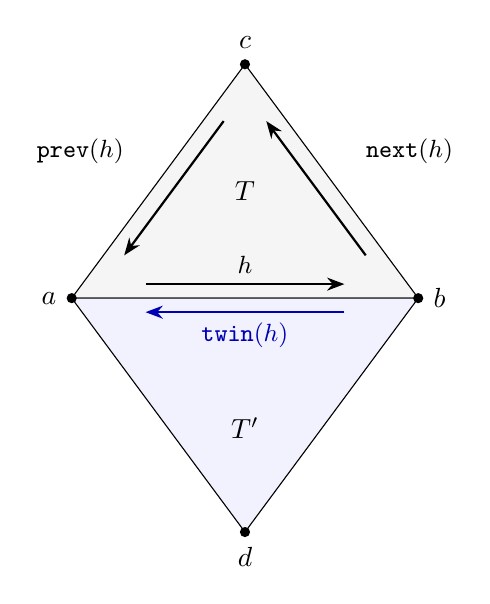
\begin{tikzpicture}[scale=2.2,
  he/.style={-{Stealth[length=2.2mm]},thick},
  tw/.style={-{Stealth[length=2.2mm]},thick,blue!70!black},
  v/.style={circle,fill=black,inner sep=1.3pt}]
  \coordinate (A) at (0,0); \coordinate (B) at (2,0); \coordinate (C) at (1,1.35); \coordinate (D) at (1,-1.35);
  \draw[fill=gray!8] (A)--(B)--(C)--cycle; \draw[fill=blue!5] (A)--(D)--(B)--cycle;
  \node[v,label=left:$a$] at (A) {}; \node[v,label=right:$b$] at (B) {};
  \node[v,label=above:$c$] at (C) {}; \node[v,label=below:$d$] at (D) {};
  \coordinate (G) at (1,0.45); % centroid of T
  \draw[he] ($(A)!0.15!(B)!0.18!(G)$) -- node[above]{\small $h$} ($(A)!0.85!(B)!0.18!(G)$);
  \draw[he] ($(B)!0.15!(C)!0.18!(G)$) -- ($(B)!0.85!(C)!0.18!(G)$);
  \draw[he] ($(C)!0.15!(A)!0.18!(G)$) -- ($(C)!0.85!(A)!0.18!(G)$);
  \node[font=\small] at (1.95,0.85) {\texttt{next}$(h)$};
  \node[font=\small] at (0.05,0.85) {\texttt{prev}$(h)$};
  \coordinate (H) at (1,-0.45); % centroid of T'
  \draw[tw] ($(B)!0.15!(A)!0.18!(H)$) -- node[below]{\small \texttt{twin}$(h)$} ($(B)!0.85!(A)!0.18!(H)$);
  \node at (1,0.62) {$T$}; \node at (1,-0.75) {$T'$};
\end{tikzpicture}
\caption{Half-edges of two neighbouring triangles. The half-edge $h$ runs from its origin $a$
to its target $b$ (\texttt{vertex\_idx} is the index of $b$); \texttt{next\_idx} cycles through
the three half-edges of $T$ in winding order; the twin runs $b\to a$ in the neighbouring
triangle $T'$. The origin of $h$ is the target of \texttt{prev}$(h)$, so it is found without
the twin.}
\label{fig:halfedge}
\end{figure}

\paragraph{Vertex} (\texttt{MFTL\_Vertex}):
\begin{itemize}
  \item \texttt{pos[3]}: the position, \emph{wrapped} into $[\min,\max)$ on periodic axes;
    \texttt{img[3]}: the periodic image counters (Chapter~\ref{ch:periodicity});
  \item derived geometry: \texttt{normal}, \texttt{meancurvature} ($2H$),
    \texttt{gaussiancurvature}, \texttt{area} (mixed Voronoi area), \texttt{roughness\_mean},
    \texttt{roughness\_variance}, and \texttt{curv\_extrap} (extrapolated curvature of a
    boundary vertex);
  \item \texttt{owner\_proc}, \texttt{is\_ghost}, \texttt{global\_id};
  \item \texttt{out\_he\_idx}: the local index of one outgoing half-edge --- the entry point of
    the one-ring walk. On a boundary vertex it is the outgoing boundary half-edge;
  \item \texttt{flags}: \texttt{MFTL\_FLAG\_*} and \texttt{MFTL\_VFLAG\_*} bits (remeshing
    marks, sharp features, curvature validity, boundary corners).
\end{itemize}

\paragraph{Triangle} (\texttt{MFTL\_Triangle}):
\begin{itemize}
  \item \texttt{he\_idx}: the local index of one of its three half-edges;
  \item cached \texttt{normal}, \texttt{area} and \texttt{center} (set by
    \fn{MFTLComputeTriangleProperties}, see \S\ref{sec:triprops});
  \item \texttt{owner\_proc}, \texttt{is\_ghost}, \texttt{global\_id}, \texttt{flags};
  \item \texttt{data}: an opaque payload of \texttt{data\_size} bytes, and
    \texttt{surface\_scalar}, a conserved concentration per unit area (Chapter~\ref{ch:data}).
\end{itemize}

\paragraph{Half-edge} (\texttt{MFTL\_HalfEdge}): a directed edge of exactly one triangle.
\begin{itemize}
  \item \texttt{vertex\_idx}: the vertex at its \emph{end} (target);
  \item \texttt{next\_idx}: the next half-edge of the same triangle in winding order; the three
    half-edges of a triangle form a cycle;
  \item \texttt{triangle\_idx}: its triangle;
  \item \texttt{twin\_idx} and \texttt{twin\_gid}: the opposite half-edge. Together they encode
    the \emph{twin state} LOCAL, REMOTE or BOUNDARY (Chapter~\ref{ch:topology}). They are
    never read directly: the predicates \fn{MFTLHeIsLocal}, \fn{MFTLHeIsRemote},
    \fn{MFTLHeIsBoundary}, \fn{MFTLHeBoundaryTag}, \fn{MFTLHeTwinGid} and \fn{MFTLHeEdgeId} are
    the only sanctioned readers (the script \texttt{tools/check\_twin\_gid\_readers.sh} enforces
    this in the library sources);
  \item \texttt{global\_id}, \texttt{flags}, and \texttt{boundary}, a cache of
    \fn{MFTLHeIsBoundary}.
\end{itemize}

\section{Navigation}

\texttt{mftl\_topology.h} provides inline accessors. With a half-edge $h$:
\fn{MFTLHeTarget} and \fn{MFTLHeOrigin} give its end and start vertex, \fn{MFTLHeNext} and
\fn{MFTLHePrev} the other half-edges of its triangle, \fn{MFTLHeTriangle} its triangle and
\fn{MFTLHeTwin} its stored twin. \fn{MFTLHeTwin} returns \texttt{NULL} when the twin is not
stored on this rank, which happens both at a physical boundary and at an MPI rim;
\texttt{NULL} must therefore never be taken to mean ``boundary''. For a triangle,
\fn{MFTLGetTriangleHalfedges} and \fn{MFTLGetTriangleVertices} return its half-edges and
vertices in winding order, and \fn{MFTLGetTriangleNeighbors} the triangles across its edges.

\paragraph{One-ring traversal.} The triangles around a vertex $v$ are visited through its
outgoing half-edges: from an outgoing half-edge $h$, the next one is
$\texttt{next}(\texttt{twin}(h))$. Seen from the side into which the triangle normals point
(from outside an outward-wound body, where the triangles appear counter-clockwise), this step
turns \emph{clockwise} around $v$, and $\texttt{twin}(\texttt{prev}(h))$ turns
counter-clockwise (Figure~\ref{fig:onering}). The walk stops where a half-edge has no stored
twin. \fn{MFTLGetVertexOneRing}, \fn{MFTLGetVertexOneRingVertices} and
\fn{MFTLGetVertexOneRingHalfedges} first rewind counter-clockwise to such a stop (unless the caller asserts a closed fan with \texttt{is\_inner}), so an
open fan is returned from one end to the other. \fn{MFTLVertexRing} classifies the fan of a
vertex as
\begin{itemize}
  \item \texttt{MFTL\_RING\_CLOSED}: an interior vertex whose whole fan is stored;
  \item \texttt{MFTL\_RING\_OPEN\_COMPLETE}: a boundary vertex; the fan runs from an incoming to
    an outgoing boundary half-edge;
  \item \texttt{MFTL\_RING\_INCOMPLETE}: the walk reaches a REMOTE half-edge (the fan is cut by
    an MPI rim) or the fan is malformed.
\end{itemize}

\begin{figure}[ht]
\centering
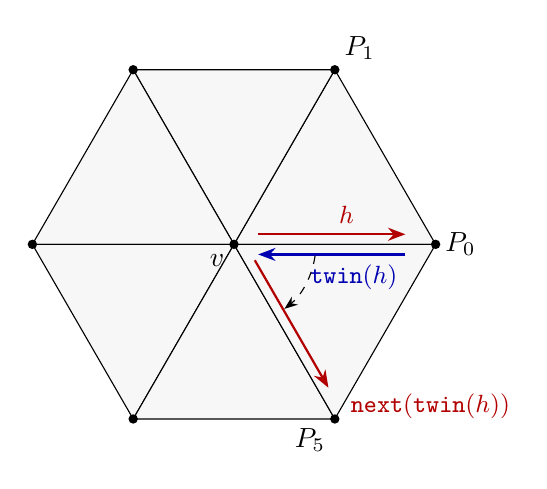
\begin{tikzpicture}[scale=1.6,
  he/.style={-{Stealth[length=2.2mm]},thick},
  v/.style={circle,fill=black,inner sep=1.2pt}]
  \coordinate (V) at (0,0);
  \foreach \i in {0,...,5} { \coordinate (P\i) at ({60*\i}:1.6); }
  \foreach \i/\j in {0/1,1/2,2/3,3/4,4/5,5/0} { \draw[fill=gray!6] (V)--(P\i)--(P\j)--cycle; }
  \foreach \i in {0,...,5} { \node[v] at (P\i) {}; }
  \node[v] at (V) {}; \node[below left] at (V) {$v$};
  \node[right] at (P0) {$P_0$}; \node[below left] at (P5) {$P_5$}; \node[above right] at (P1) {$P_1$};
  % seen from the normal side: triangles are counter-clockwise, so h = v->P0 lies in (v,P0,P1)
  \draw[he,red!70!black] ($(V)!0.12!(P0)+(90:0.08)$) -- node[above,pos=0.6]{\small $h$} ($(V)!0.85!(P0)+(90:0.08)$);
  % twin(h) = P0->v lies in (v,P5,P0)
  \draw[he,blue!70!black] ($(P0)!0.15!(V)+(-90:0.08)$) -- node[below,pos=0.35]{\small \texttt{twin}$(h)$} ($(P0)!0.88!(V)+(-90:0.08)$);
  % next(twin(h)) = v->P5, also in (v,P5,P0)
  \draw[he,red!70!black] ($(V)!0.12!(P5)+(30:0.08)$) -- ($(V)!0.85!(P5)+(30:0.08)$);
  \node[red!70!black,right] at ($(P5)+(0.05,0.1)$) {\small \texttt{next}(\texttt{twin}$(h)$)};
  \draw[-{Stealth},dashed] (-8:0.65) arc (-8:-52:0.65);
\end{tikzpicture}
\caption{The one-ring of $v$, seen from the side the normals point to (triangles
counter-clockwise). Red: the outgoing half-edges $h=v\to P_0$ and $\texttt{next}(\texttt{twin}(h))
=v\to P_5$; blue: $\texttt{twin}(h)$. The walk $h\mapsto\texttt{next}(\texttt{twin}(h))$ turns
clockwise around $v$.}
\label{fig:onering}
\end{figure}

\section{Flattened connectivity and neighbourhoods}

Some kernels (the LBVH, the neighbourhood search, the remesher's fits) use compact
connectivity arrays built by \fn{MFTLFlattenConnectivity}:
\texttt{flat\_tri\_verts[3t+j]} is the target vertex of the $j$-th half-edge of triangle $t$,
\texttt{flat\_tri\_neighbors[3t+j]} the triangle across that half-edge ($-1$ if its twin is
not stored), and \texttt{vert\_offsets}/\texttt{vert\_tris} a CSR map from a vertex to its
incident stored triangles. The generators, readers, builders and the redistribution rebuild
them; an application that calls the topological operators of the remesher directly calls
\fn{MFTLFlattenConnectivity} itself afterwards. \fn{MFTLGetNeighborhood} gathers vertices and triangles
breadth-first on this incidence graph (one step from a vertex gives its triangles, two steps
also their vertices).

\section{Owned entities first}

After a redistribution on more than one rank the owned entities of every array come first
and the ghosts follow; \texttt{n\_local\_vertices}, \texttt{n\_local\_triangles} and
\texttt{n\_local\_half\_edges} are then the lengths of the owned prefixes. These counts are set
only by a multi-rank redistribution, the builders (soups, \fn{MFTLBuildTopologyFromTriples}), the
staged copy \fn{MFTLObjectAppendTriangleCopy} and \fn{MFTLObjectClear};
generators, remeshing and a single-rank redistribution (which does nothing) do not update
them. Code that must work in every state therefore loops over the stored arrays and skips
entities with \texttt{is\_ghost} set --- the library itself identifies owned entities this way,
and so do all the examples in this manual.

\section{Global counts and id counters}

\texttt{global\_n\_triangles} and \texttt{global\_n\_vertices} of an object are the numbers of owned
entities summed over all ranks; they are refreshed by the collective
\fn{MFTLEnsembleUpdateGlobalCounts} (all objects) or \fn{MFTLObjectUpdateGlobalStats} (one
object). The counters \texttt{next\_vertex\_gid}, \texttt{next\_triangle\_gid} and
\texttt{next\_halfedge\_gid} hold the next unused global ids and are identical on every rank;
the parallel remesher hands out disjoint per-rank blocks of ids and re-synchronises the
counters afterwards (\fn{MFTLSyncEnsembleGidCounters}).

\chapter{The parallel model}
\label{ch:parallel}

\section{Decomposition}

The global box $[\vect{x}_{\min},\vect{x}_{\max})$ is divided into
$\texttt{cuts[0]}\times\texttt{cuts[1]}\times\texttt{cuts[2]}$ sub-boxes, one per rank. With
\fn{MFTLEnsembleCreate} the division is uniform and sub-box $(i,j,k)$ belongs to the rank that
the MPI Cartesian communicator assigns to it; with \fn{MFTLEnsembleCreateRectilinear} the slab
coordinates along every axis (\texttt{axis\_cuts}) and the map from sub-box to rank
(\texttt{rank\_map}) are given explicitly. The domain stores the box, its size
$\vect{L}=\vect{x}_{\max}-\vect{x}_{\min}$ (\texttt{domain\_size}), half of it
(\texttt{domain\_half\_size}, the minimum-image threshold), the periodicity per axis, and the
de-duplicated list of the ranks owning the up to 26 neighbouring sub-boxes
(\texttt{neighbors}). On a periodic axis with one or two slabs a rank may be its own
neighbour, or the same rank may be the neighbour on both sides; the library handles both.

The owner of a point is the rank of the sub-box that contains it:
\begin{lstlisting}[numbers=none]
static inline int MFTLGetOwnerProc(const MFTL_Domain *domain, const double pos[3]);
\end{lstlisting}
Points on an internal slab face belong to the upper slab; points outside the box are clamped
to the first or last slab. During load-balanced remeshing a temporary x-only ownership
(\texttt{lb\_nprocs}, \texttt{lb\_xcuts}) replaces the Cartesian map (\S\ref{sec:parallel-remesh}).

\section{Ownership}

Every entity has exactly one owner, the only rank whose copy is authoritative:
\begin{itemize}
  \item a \emph{vertex} is owned by the rank that owns its position \texttt{pos};
  \item a \emph{triangle} is owned by the rank that owns its \emph{cached} centre
    \texttt{center} (the centroid of its corners, wrapped into the box);
  \item a \emph{half-edge} belongs to its triangle.
\end{itemize}
Copies on other ranks are \emph{ghosts}: \texttt{is\_ghost} is set and \texttt{owner\_proc} names
the owner. Ghosts are read-only: they exist so that the owner of a vertex can see the whole fan
around it and so that the owner of a triangle can see its neighbours. A value written into a
ghost is overwritten at the next refresh. Integrals and statistics count owned entities only.

Because the triangle owner is taken from the cached centre, \fn{MFTLComputeTriangleProperties}
must be called after positions have changed and before a redistribution. The transforms of
Chapter~\ref{ch:geometry} and the remesher do this themselves; an application that moves
vertices itself calls it explicitly (see the listings of Chapter~\ref{ch:examples}).

\section{Redistribution}

\begin{lstlisting}[numbers=none]
int MFTLRedistribute(MFTL_Ensemble *ens);             /* all objects of the ensemble */
int MFTLRedistributeObject(MFTL_Object *object);      /* one object */
int MFTLRedistributeListOfObjects(MFTL_Ensemble *ensemble);
\end{lstlisting}
A redistribution (collective) recomputes the owner of every entity from its current position
(vertices) or cached centre (triangles) and moves it there. Each triangle is sent to its owner,
to the owners of its three vertices and to the owners of its edge-neighbour triangles, so every
rank receives one layer of ghosts around its owned part (Figure~\ref{fig:distribution}). Global
ids, image counters, flags, the cached triangle geometry, the surface scalar and the opaque
payload travel with the entities; local indices are rebuilt.

On return the ensemble is at a \emph{quiescent point}:
\begin{itemize}
  \item every entity is owned exactly once, and the owned entities are stored first;
  \item every edge of an owned triangle is LOCAL or BOUNDARY (ghost completion G1) and the
    fan of every owned vertex is stored completely (G2), \S\ref{sec:completion};
  \item the twin states have been validated (\S\ref{sec:validation}).
\end{itemize}
On a single rank a redistribution does nothing and returns \texttt{MFTL\_SUCCESS}. It returns
\texttt{MFTL\_ERROR} on a payload-size mismatch between ranks or when ghost completion or
validation fails. \fn{MFTLRedistribute} calls \fn{MFTLRedistributeObject} for an ensemble with
one object and \fn{MFTLRedistributeListOfObjects} otherwise; the latter moves all objects in
one communication round.

\begin{figure}[ht]
\centering
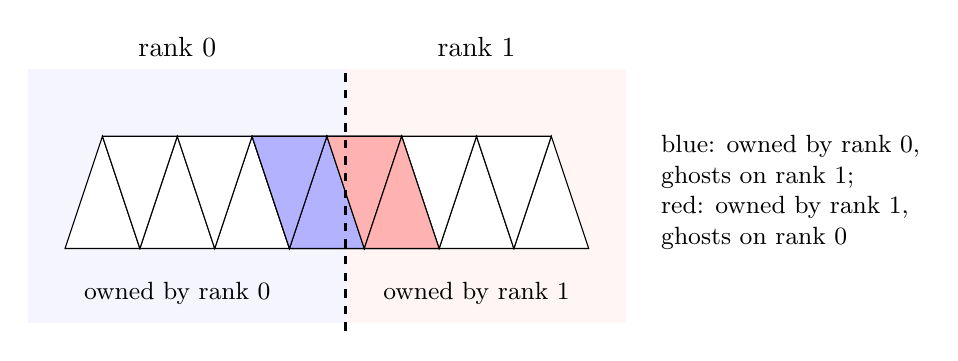
\begin{tikzpicture}[scale=0.95]
  \fill[blue!4] (0,0) rectangle (4.25,3.4); \fill[red!4] (4.25,0) rectangle (8,3.4);
  \node at (2,3.7) {rank 0}; \node at (6,3.7) {rank 1};
  % strip: bottom vertices (x,1), top vertices (x+0.5,2.5); up-triangles i, down-triangles i
  \foreach \x in {0.5,1.5,...,6.5} { \filldraw[fill=white,draw=black] (\x,1) -- (\x+1,1) -- (\x+0.5,2.5) -- cycle; }
  \foreach \x in {0.5,1.5,...,5.5} { \filldraw[fill=white,draw=black] (\x+0.5,2.5) -- (\x+1.5,2.5) -- (\x+1,1) -- cycle; }
  % triangles next to the slab face: owned left of it (blue), right of it (red); each stored on both ranks
  \filldraw[fill=blue!30,draw=black] (3.5,1) -- (4.5,1) -- (4,2.5) -- cycle;
  \filldraw[fill=blue!30,draw=black] (3,2.5) -- (4,2.5) -- (3.5,1) -- cycle;
  \filldraw[fill=red!30,draw=black] (4,2.5) -- (5,2.5) -- (4.5,1) -- cycle;
  \filldraw[fill=red!30,draw=black] (4.5,1) -- (5.5,1) -- (5,2.5) -- cycle;
  \draw[very thick,dashed] (4.25,-0.1) -- (4.25,3.4);
  \node[font=\small] at (2,0.4) {owned by rank 0};
  \node[font=\small] at (6,0.4) {owned by rank 1};
  \node[align=left,font=\small] at (10.2,1.75) {blue: owned by rank 0,\\ ghosts on rank 1;\\ red: owned by rank 1,\\ ghosts on rank 0};
\end{tikzpicture}
\caption{Distribution with one ghost layer. A triangle is owned by the rank containing its
centre; the triangles next to the slab face are also stored on the other rank as ghosts, so
that each rank sees the complete fan of every vertex it owns.}
\label{fig:distribution}
\end{figure}

\section{Refreshing ghosts}

Moving owned vertices leaves the ghost copies on other ranks stale. Two collective refreshes
update ghosts without changing which entities are stored:
\begin{itemize}
  \item \fn{MFTLUpdateGhostPositions}\texttt{(ens, lookup)} copies, for every ghost vertex, the
    owner's position, image counters, normal, curvatures, area and roughness;
  \item \fn{MFTLScatterTriangleData}\texttt{(ens, lookup)} copies the owner's opaque payload into
    every ghost triangle (Chapter~\ref{ch:data}).
\end{itemize}
Both exchange data with the graph neighbours only. A ghost whose owner is not a graph neighbour
any more (because a vertex moved further than a slab, or during parallel remeshing) stays stale
until the next redistribution; the call prints how many such ghosts it met. The argument
\texttt{lookup} is an optional hash map from object id to object index (\texttt{MFTL\_NULL}:
linear search).

Cached triangle properties of ghost triangles are \emph{not} refreshed by either call: they are
set by the owner and travel with the triangle at the next redistribution. The recommended
sequence after moving vertices is therefore
\begin{lstlisting}[numbers=none]
/* move owned vertices ... */
MFTLUpdateGhostPositions(ens, MFTL_NULL);   /* ghost vertices follow their owners      */
MFTLComputeTriangleProperties(obj);         /* cached area/normal/centre of owned tris */
MFTLRedistribute(ens);                      /* new owners, fresh ghost layer           */
\end{lstlisting}

\section{Additional ghost layers and spatial ghosts}

\fn{MFTLExtendGhostLayer}\texttt{(ens, steps)} imports further rings of ghost triangles
(\texttt{steps} layers) around the owned part, for kernels with a wider stencil than the one-ring.
Two functions import triangles by proximity rather than by topology:
\fn{MFTL\_CreateSpatialGhosts}\texttt{(objA, objB)} ships the owned triangles of one object whose
box meets the other object's box on a neighbour rank (periodic-aware box tests; used by the
intersection driver, \S\ref{sec:intersection}), and
\fn{MFTLEnsembleCreateSpatialGhosts}\texttt{(ens, tol)} ships owned triangles whose box, inflated by
\texttt{tol}, overlaps a neighbour rank's box (a plain box test on the stored positions, not
periodic-aware). \fn{MFTLObjectSendLocalTrianglesToAll}\texttt{(obj, distance)} makes every owned
triangle a ghost on \emph{every} rank whose box lies within \texttt{distance} of it (a global
exchange, not limited to the graph neighbours).

\section{Collective discipline}

Every collective function must be entered by all ranks of the ensemble in the same order.
Functions whose result depends on a point or a parameter (point queries, phase-set queries,
remesh parameters) require the same value on every rank. Inside the library, decisions that end loops or select algorithms are reduced over all ranks
before they are taken, so that no rank leaves a sequence of collectives early (see, for example,
the volume recovery of \S\ref{sec:volume-recovery}). One known defect violates this rule
(\S\ref{sec:known-defects}).

\chapter{Topology: twin states, boundaries and loops}
\label{ch:topology}

\section{The three twin states}

A triangle mesh distributed over ranks has three kinds of ``edges without a stored
neighbour'' that must never be confused: the physical boundary of an open surface, the edge of
this rank's part of the mesh (the MPI rim), and --- on a periodic domain --- the crossing of a
periodic face. \mftl{} separates them by giving every half-edge exactly one of three
\emph{twin states} at every quiescent point:

\begin{center}\small
\begin{tabular}{@{}llll@{}}
\toprule
State & \texttt{twin\_idx} & \texttt{twin\_gid} & Meaning \\
\midrule
LOCAL & $\ge 0$ & global id of the stored twin & the twin is stored on this rank \\
REMOTE & $-1$ & $\ge 0$: global id of the twin & the twin lives on another rank (MPI rim) \\
BOUNDARY & $-1$ & $-2-\text{tag}$, $\text{tag}\ge0$ & a physical boundary edge with a tag \\
\bottomrule
\end{tabular}
\end{center}

\texttt{MFTL\_TWIN\_NONE} is $-2$, so the boundary code of tag $t$ is
$\fn{MFTLBoundaryCode}(t)=-2-t$. The transient value \texttt{MFTL\_TWIN\_UNKNOWN} ($-1$) is legal
only inside an operation (a remesh pass, a staged copy) and is rejected by validation. The
states are read with the predicates of \texttt{mftl\_topology.h} only:

\begin{lstlisting}[numbers=none]
bool MFTLHeIsLocal(const MFTL_HalfEdge *he);
bool MFTLHeIsRemote(const MFTL_HalfEdge *he);
bool MFTLHeIsBoundary(const MFTL_HalfEdge *he);
int  MFTLHeBoundaryTag(const MFTL_HalfEdge *he);                 /* BOUNDARY only */
int  MFTLHeTwinGid(const MFTL_Object *obj, const MFTL_HalfEdge *he); /* -1 for BOUNDARY */
int  MFTLHeEdgeId(const MFTL_Object *obj, const MFTL_HalfEdge *he);  /* undirected edge id */
\end{lstlisting}
\fn{MFTLHeEdgeId} is the rank-independent id of the undirected edge: the smaller of the two
half-edge ids for LOCAL and REMOTE edges, the half-edge's own id for a boundary edge.

\section{Boundary, rim and seam}
\label{sec:bound-rim-seam}

Table~\ref{tab:brs} states the distinction precisely. No coordinate is ever consulted to decide
it: the physical boundary is a property of the topology, the rim a property of the
distribution, and the seam a property of the image counters.

\begin{table}[ht]
\centering\small
\begin{tabularx}{\textwidth}{@{}lXX@{}}
\toprule
Concept & Representation & Determined by \\
\midrule
Physical boundary & BOUNDARY half-edge (\texttt{twin\_idx} $=-1$, \texttt{twin\_gid} $\le -2$) & the topology only: builders, commits, remesh operators \\
MPI rim & REMOTE half-edge (\texttt{twin\_idx} $=-1$, \texttt{twin\_gid} $\ge0$), with a live twin on another rank & the ownership and ghosting only \\
Periodic seam & ordinary LOCAL or REMOTE twins; the crossing shows only in the edge lattice shift derived from the image counters (\S\ref{sec:winding}) & the topology plus the counters \\
\bottomrule
\end{tabularx}
\caption{Physical boundary, MPI rim and periodic seam.}
\label{tab:brs}
\end{table}

The concepts compose: an edge across a periodic seam may also be an MPI rim; a physical
boundary may run across seams and rank boundaries --- its half-edges are BOUNDARY on every rank,
and its loop is built collectively (\S\ref{sec:loops}).

\begin{figure}[ht]
\centering
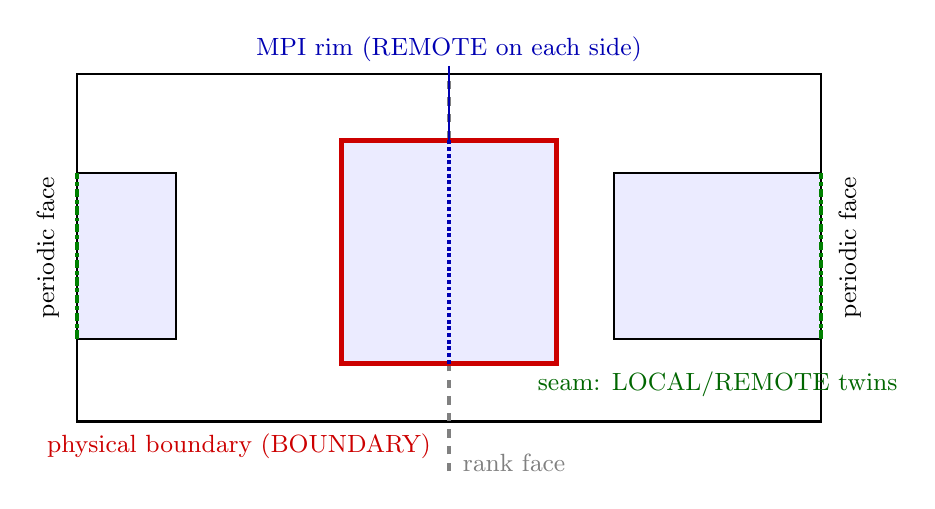
\begin{tikzpicture}[scale=1.05]
  \draw[thick] (0,0) rectangle (9,4.2);
  \draw[very thick,dashed,gray] (4.5,-0.6) -- (4.5,4.2); \node[gray,font=\small,right] at (4.55,-0.5) {rank face};
  \node[font=\small] at (-0.35,2.1) [rotate=90] {periodic face};
  \node[font=\small] at (9.35,2.1) [rotate=90] {periodic face};
  % an open patch crossing the rank face and the periodic face
  \draw[fill=blue!8,thick] (6.5,1) -- (9,1) -- (9,3) -- (6.5,3) -- cycle;
  \draw[fill=blue!8,thick] (0,1) -- (1.2,1) -- (1.2,3) -- (0,3) -- cycle;
  \draw[fill=blue!8] (3.2,0.7) -- (5.8,0.7) -- (5.8,3.4) -- (3.2,3.4) -- cycle;
  \draw[red!80!black,line width=1.6pt] (3.2,0.7) -- (5.8,0.7) -- (5.8,3.4) -- (3.2,3.4) -- cycle;
  \draw[blue!70!black,line width=1.4pt,densely dotted] (4.5,0.7) -- (4.5,3.4);
  \draw[green!50!black,line width=1.4pt,densely dashdotted] (9,1) -- (9,3); \draw[green!50!black,line width=1.4pt,densely dashdotted] (0,1) -- (0,3);
  \node[font=\small,red!80!black,left] at (4.4,-0.3) {physical boundary (BOUNDARY)};
  \node[font=\small,blue!70!black] at (4.5,4.5) {MPI rim (REMOTE on each side)};
  \draw[blue!70!black,thin] (4.5,4.3) -- (4.5,3.4);
  \node[font=\small,green!40!black,align=center] at (7.75,0.45) {seam: LOCAL/REMOTE twins};
\end{tikzpicture}
\caption{The three situations in which a rank stores no twin across an edge, or in which an
edge crosses the box: a physical boundary (a tagged BOUNDARY half-edge), an MPI rim (REMOTE
half-edges whose twins live on the neighbouring rank) and a periodic seam (ordinary twins; the
crossing is visible only through the image counters).}
\label{fig:brs}
\end{figure}

\section{Declared class: closed and open bodies}

A body is closed unless the application declares it open, identically on every rank, before
it is built:
\begin{lstlisting}[numbers=none]
void MFTLObjectDeclareOpen(MFTL_Object *obj, int open);
\end{lstlisting}
Only a declared-open body may have BOUNDARY half-edges. An unmatched edge in the input of a
closed body is an error, never a silently created boundary. The declared class, the boundary
tags and the image counters are the only information from which the library derives what a
body is; geometric proximity to the box faces plays no role.

\section{Building a mesh}

\paragraph{From vertex positions and index triples (rank-local).}\mbox{}
\begin{lstlisting}[numbers=none]
int MFTLBuildTopologyFromTriples(MFTL_Object *obj, int nV, const double positions[][3],
                                 int nF, const int triples[][3]);
\end{lstlisting}
For a triple $(a,b,c)$ the three half-edges target $b$, $c$ and $a$ and cycle in that order, so
the winding of the triples defines the orientation. Twins are paired locally; on a declared-open
body every unpaired half-edge becomes BOUNDARY, with tags numbering the boundary loops in the
order of their smallest vertex id; on a closed body an unpaired half-edge is an error. Duplicate
directed half-edges (a non-manifold edge, inconsistent orientation, a M\"obius strip) and bow-tie
vertices are rejected. Positions are stored as given with \texttt{img} $=0$; a caller with
continuous coordinates wraps them first. The generators and the readers use this path.

\paragraph{From a distributed triangle soup (collective).}\mbox{}
\begin{lstlisting}[numbers=none]
int MFTLBuildFromSoup(MFTL_Object *obj, int nV, const int *vgid, const double (*pos)[3],
                      const int *vowner, int nT, const int *tgid, const int (*tvg)[3],
                      const int *towner);
int MFTLBuildFromSoupEx(/* as above */ ..., const MFTL_BoundaryDecl *decl);
int MFTLBuildFromSoupImg(/* wrapped positions with image counters */ ...);
\end{lstlisting}
Every rank passes the vertices and triangles it knows, with global ids; a triangle names its
vertices by global id, and the order of its three vertex ids defines its orientation. An
entity may be passed on several ranks (with identical data). Twins are paired locally, then
every unpaired half-edge is resolved \emph{globally} across ranks: if the twin exists anywhere,
the half-edge becomes REMOTE. An edge that is unmatched everywhere becomes BOUNDARY only if the
body is declared open \emph{and} the boundary declaration names it:

\begin{lstlisting}[numbers=none]
typedef struct MFTL_BoundaryEdgeDecl { int vgid_a, vgid_b; int tag; } MFTL_BoundaryEdgeDecl;
typedef struct MFTL_BoundaryDecl {
  int from_mesh;   /* "BoundaryFromMesh": every edge unmatched on every rank is a boundary */
  int n_edges;     /* or an explicit list of boundary edges with tags (union over ranks)  */
  const MFTL_BoundaryEdgeDecl *edges;
} MFTL_BoundaryDecl;
\end{lstlisting}
With \texttt{from\_mesh} the loops are tagged automatically in the order of their smallest vertex
id. Any other unmatched edge, a declared edge that is not unmatched, or a duplicate directed
half-edge is a collective error. All entities are stored with the given owners (\texttt{NULL}:
this rank); a redistribution establishes the real ownership. The example of
\S\ref{sec:ex-open} builds an open patch this way.

\paragraph{Staged copies.} \fn{MFTLObjectAppendTriangleCopy} copies a triangle (with its
half-edges, missing vertices, payload and surface scalar) from one object into another. The copy
is \emph{staged}: half-edges whose twin was not copied keep the source's state code, and the
destination is not quiescent until the batch is closed by the collective
\fn{MFTLObjectCommitCopy}\texttt{(dst, mode)}. With \texttt{MFTL\_COMMIT\_ASSEMBLE} every such
half-edge must find its twin among the destination's authoritative half-edges on some rank;
with \texttt{MFTL\_COMMIT\_CUT} the half-edges whose source twin was not copied become BOUNDARY
with one new tag (the destination must be declared open). \multi{} uses this to split a body
into its connected components (breakup) and to merge bodies (coalescence).

\section{Validation}
\label{sec:validation}

\begin{lstlisting}[numbers=none]
int MFTLCheckMeshIntegrity(MFTL_Object *object);                 /* rank-local */
int MFTLCheckTwinStatesLocal(const MFTL_Object *obj, int flags, int verbose);
int MFTLValidateTwinStatesEx(MFTL_Object *obj, int flags);       /* collective */
int MFTLValidateTwinStates(MFTL_Object *obj);
\end{lstlisting}
\fn{MFTLCheckMeshIntegrity} checks index bounds, triangle cycles, twin symmetry and vertex
consistency. \fn{MFTLCheckTwinStatesLocal} checks, rank-locally, that every live half-edge has a
legal state, that LOCAL pairs are symmetric, that only declared-open bodies have BOUNDARY
half-edges, that no directed half-edge is duplicated, and the boundary-vertex conventions; with
\texttt{MFTL\_VALIDATE\_GHOSTS} it also checks G1 and G2. \fn{MFTLValidateTwinStates} adds the
collective \emph{remote liveness} check: every REMOTE twin id is held as a live authoritative
half-edge on some rank that names the requester back, and every boundary edge carries the same
tag on every rank that stores it.

The library runs a check at every quiescent point (after builds and commits, redistribution,
remesh finalisation, the end of a serial bracket, and reading a native mesh): the full
collective validation in Debug builds or when \texttt{MFTL\_VALIDATE} is set, the cheap local
checks otherwise.

\section{Remote-twin discovery and ghost completion}
\label{sec:completion}

When a rank holds a REMOTE half-edge it knows the global id of the twin but not where it lives.
Two discovery modes find it:
\begin{itemize}
  \item \emph{Global mode} (before ownership exists: builders, commits, and as a fallback): the
    requested ids are gathered on every rank, and any rank holding a live authoritative copy
    answers.
  \item \emph{Owned mode} (after a redistribution): the twin triangle's centroid lies within
    $\ell_{\max}/3$ of the edge midpoint ($\ell_{\max}$: the longest edge), so the request goes to
    the ranks whose box meets the (periodic) ball of radius $\ell_{\max}/3+2\varepsilon$ around
    the midpoint, $\varepsilon$ being a margin for stale ghost positions. The global mode then
    always runs as a fallback (it carries no data when the first round was complete).
\end{itemize}
\fn{MFTLCompleteGhosts}, called by every redistribution, uses the discovery to import the missing
neighbours as ghosts until the two guarantees hold:
\begin{description}
  \item[G1] every edge of every owned triangle is LOCAL or BOUNDARY;
  \item[G2] the complete fan of every owned vertex is stored.
\end{description}
Kernels that work on the one-ring of an owned vertex (normals, curvature, smoothing) rely on G2;
kernels that look across the edges of an owned triangle rely on G1. Ghost triangles themselves
may keep REMOTE edges.

\section{Boundary vertices, tags and loops}
\label{sec:loops}

A \emph{boundary vertex} has exactly one outgoing and one incoming BOUNDARY half-edge; its
\texttt{out\_he\_idx} points at the outgoing one, so the loop is walked from vertex to vertex.
Tags are persistent handles for the parts of the boundary: splits inherit the tag of the split
edge, collapses along a boundary keep it, and a CUT commit creates a new one. \multi{} attaches
its boundary conditions to them (\S\ref{sec:mf-bcs}).

\begin{lstlisting}[numbers=none]
typedef struct MFTL_BoundaryLoop {
  int n;              /* number of boundary edges (= vertices) */
  int *edge_ids;      /* in loop order; edge i runs vertex_gids[i] -> vertex_gids[i+1] */
  int *vertex_gids;
  int tag;            /* the smallest tag when mixed */
  int mixed_tags;
  double length;      /* sum of minimum-image edge lengths */
  int winding[3];     /* sum of the edge lattice shifts around the loop */
} MFTL_BoundaryLoop;
int  MFTLBoundaryLoops(MFTL_Object *obj, MFTL_BoundaryLoopSet *out);   /* collective */
void MFTLFreeBoundaryLoops(MFTL_BoundaryLoopSet *set);
\end{lstlisting}
\fn{MFTLBoundaryLoops} collects one record per owned boundary vertex (its incoming and outgoing
edge ids, its id, the tag and the outgoing edge's length and lattice shift), gathers the
records on every rank and chains them into loops, ordered by their smallest vertex id. The
result is identical on every rank and independent of the rank count and of seams. It needs G2
(call it after a redistribution, or on one rank). A non-zero winding vector means the loop
itself spans a periodic direction (\S\ref{sec:winding}).

The orientation of a loop follows the half-edges: on an outward-facing patch, walking along
the boundary half-edges keeps the surface on the left. \fn{MFTLBoundaryEdgeGeometry} returns, for
a boundary half-edge, its length $L_e$, the unit tangent $\vect{t}$ along it, the in-surface
outward \emph{conormal} $\vect{\nu}=\vect{t}\times\vect{n}$ ($\vect{n}$: the unit normal of its
triangle) and the continuous midpoint (Figure~\ref{fig:conormal}).

\begin{figure}[ht]
\centering
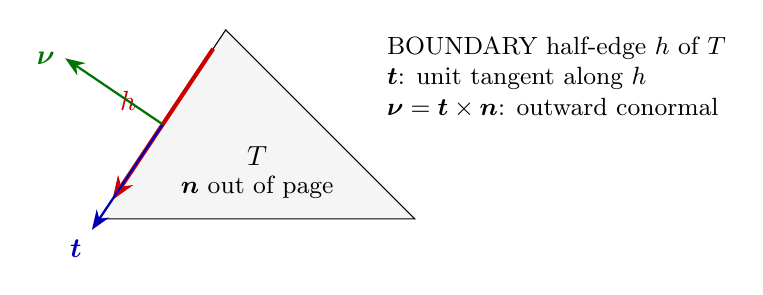
\begin{tikzpicture}[scale=2]
  \coordinate (A) at (0,0); \coordinate (B) at (2,0); \coordinate (C) at (0.8,1.2);
  \draw[fill=gray!8] (A)--(B)--(C)--cycle;
  \draw[red!80!black,line width=1.5pt,-{Stealth[length=3mm]}] ($(C)!0.1!(A)$) -- ($(C)!0.9!(A)$);
  \node[red!80!black] at (0.18,0.75) {$h$};
  \coordinate (M) at ($(C)!0.5!(A)$);
  \draw[-{Stealth[length=2.5mm]},thick,blue!70!black] (M) -- ++(-0.45,-0.67) node[below left] {$\vect{t}$};
  \draw[-{Stealth[length=2.5mm]},thick,green!45!black] (M) -- ++(-0.62,0.42) node[left] {$\vect{\nu}$};
  \node at (1,0.4) {$T$}; \node[font=\small] at (1,0.2) {$\vect{n}$ out of page};
  \node[font=\small,align=left] at (2.9,0.9) {BOUNDARY half-edge $h$ of $T$\\ $\vect{t}$: unit tangent along $h$\\ $\vect{\nu}=\vect{t}\times\vect{n}$: outward conormal};
\end{tikzpicture}
\caption{Geometry of a boundary edge (\fn{MFTLBoundaryEdgeGeometry}).}
\label{fig:conormal}
\end{figure}

\chapter{Periodicity and image counters}
\label{ch:periodicity}

\section{Wrapped positions and continuous coordinates}

On a periodic axis $k$ with period $L_k$ every vertex position is stored \emph{wrapped} into
$[x_{\min,k},x_{\max,k})$. A surface that crosses the periodic face is therefore stored in pieces
at both ends of the box, although it is one connected mesh. To know where each vertex lies on
the unbroken surface, every vertex carries integer \emph{image counters} \texttt{img[3]}, and its
\emph{continuous coordinate} is
\begin{equation}
  \vect{X} = \texttt{pos} + \texttt{img}\odot\vect{L},
  \label{eq:continuous}
\end{equation}
with $\texttt{img}_k=0$ on non-periodic axes. \fn{MFTLVertexContinuous} evaluates
(\ref{eq:continuous}). For vertices with large counters the library never forms $\vect{X}$ inside
sums; it uses coordinates relative to a reference vertex, with the integer part exact:
\begin{equation}
  \vect{Y} = (\texttt{img}-\texttt{img}_{\text{ref}})\odot\vect{L} + (\texttt{pos}-\texttt{pos}_{\text{ref}})
  \qquad (\fn{MFTLVertexRelative}).
\end{equation}

\section{Minimum image and the edge-length restriction}

The only geometric restriction is local: \textbf{every edge is shorter than half a period} on
every periodic axis. Then the difference of the wrapped positions of the two ends of an edge,
reduced by one period where it exceeds half a period, is the true edge vector:
\begin{equation}
  d_k(u,v) = \Delta_k - L_k\,[\Delta_k > L_k/2] + L_k\,[\Delta_k < -L_k/2],\qquad
  \Delta_k = \texttt{pos}_{v,k}-\texttt{pos}_{u,k}
  \label{eq:minimage}
\end{equation}
(\fn{MFTLGetMinimumImageVector}). Every local kernel --- triangle properties, curvature, fits,
smoothing, boundary geometry --- works with minimum-image differences from an anchor vertex, so a
triangle across a seam is treated exactly like one in the middle of the box.
\fn{MFTLCheckMinimumImageConstraint} (collective) checks the edge restriction; there is no
restriction on the size of a body.

\section{Keeping the counters right}
\label{sec:displacement}

The counters stay meaningful because every vertex update follows one \emph{displacement rule}:
a vertex moves by a displacement shorter than half a period from an anchor with a known
continuous coordinate, and the new position is wrapped with the wrap counted into
\texttt{img}. The helpers in \texttt{mftl\_geometry.h} implement the cases:
\begin{description}
  \item[\fn{MFTLWrapPosImg}\texttt{(dom, pos, img)}] wraps a position that moved by less than one
    period and counts the wrap: $\texttt{pos}\mathrel{-}=L_k$, $\texttt{img}_k\mathrel{+}=1$ above the box,
    and the reverse below. The continuous coordinate is unchanged.
  \item[\fn{MFTLImgFollow}\texttt{(dom, img, old, new)}] updates the counters when a wrapped position
    is \emph{replaced} by an independently wrapped value (a fit, a smoothing result): the move is
    taken as the minimum-image displacement.
  \item[\fn{MFTLWrapContinuous}\texttt{(dom, X, pos, img)}] turns a continuous input coordinate
    into $(\texttt{pos},\texttt{img})$ with $\texttt{img}_k=\lfloor (X_k-x_{\min,k})/L_k\rfloor$.
  \item[\fn{MFTLWrapObjectIntoDomain}\texttt{(obj)}] wraps all owned vertices of a body, counting
    every wrap.
\end{description}
\fn{MFTLApplyPeriodicity} wraps a bare point (for example a query point); it must not be used on
a vertex, because it does not count the wrap.

Table~\ref{tab:imglife} lists how the library maintains the counters.

\begin{table}[ht]
\centering\small
\begin{tabularx}{\textwidth}{@{}lX@{}}
\toprule
Event & Counter rule \\
\midrule
Continuous input (generators, GTS files) & $\texttt{img}=\lfloor(\vect{X}-\vect{x}_{\min})\oslash\vect{L}\rfloor$, then canonicalisation \\
Wrapped input without counters (native v1 files, soups) & $\texttt{img}=0$, then canonicalisation assigns consistent counters \\
Translation by the application or \fn{MFTLTranslateObject} & positions move without wrapping; \fn{MFTLWrapObjectIntoDomain} wraps and counts \\
Scaling, rotation (\fn{MFTLScaleObject}, \fn{MFTLRotateObject}) & continuous coordinates relative to the body reference point, then wrap \\
Split of an edge $a\to b$ & the new vertex is placed from anchor $a$ by the minimum-image displacement \\
Collapse, fits, smoothing, volume recovery & displacement rule from the vertex's own anchor \\
Flip & no vertex changes \\
Redistribution, ghost refresh & \texttt{img} travels with \texttt{pos} \\
Native mesh v2 / restart & stored and restored exactly \\
\bottomrule
\end{tabularx}
\caption{Lifecycle of the image counters.}
\label{tab:imglife}
\end{table}

\section{Winding and canonicalisation}
\label{sec:winding}

\paragraph{Edge lattice shift.} For an edge $u\to v$ and a periodic axis $k$, the integer
\begin{equation}
  s_k(u,v) = \operatorname{round}\!\left(\frac{X_{v,k}-X_{u,k}-d_k(u,v)}{L_k}\right)
  = \texttt{img}_{v,k}-\texttt{img}_{u,k}+j_k,
  \label{eq:shift}
\end{equation}
where $j_k\in\{-1,0,1\}$ is the wrap in (\ref{eq:minimage}), measures how many periods the
continuous coordinates jump along the edge (\fn{MFTLEdgeShift}). An edge with $s_k\neq0$ is a
\emph{cut edge} along $k$.

\paragraph{Winding.} Around any closed cycle $\gamma$ of mesh edges the minimum-image
displacements add up to the true displacement around the cycle, which is $L_k W_k(\gamma)$ with
\begin{equation}
  W_k(\gamma) = \sum_{e\in\gamma} s_k(e).
\end{equation}
A connected component \emph{winds} (wraps) along $k$ if some cycle has $W_k\neq0$ --- the surface
closes on itself only after going once (or more) around the period. This is a topological
property of the embedded surface; it does not depend on the values of the counters. A sphere
across a seam does not wind; a ribbon spanning the box along $x$ winds along $x$; a flat film
spanning $x$ and $y$ winds along both (Figure~\ref{fig:winding}).

\begin{figure}[ht]
\centering
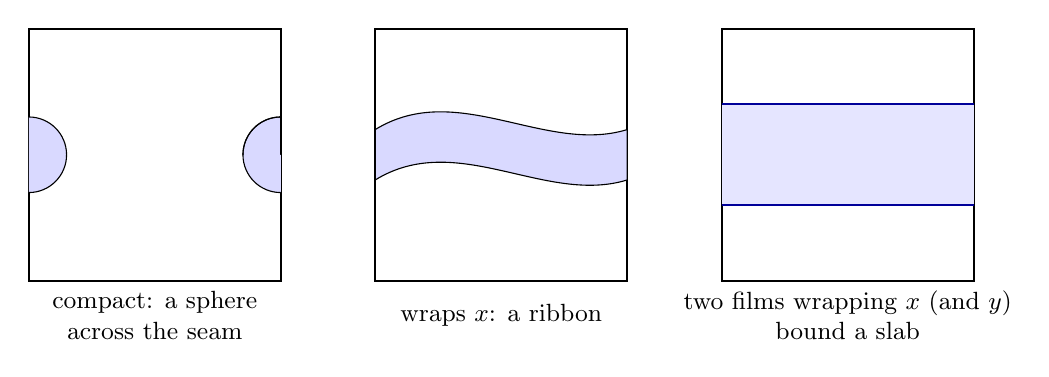
\begin{tikzpicture}[scale=0.8]
  \begin{scope}
    \draw[thick] (0,0) rectangle (4,4);
    \draw[fill=blue!15] (4,2) ++(-0.6,0) arc (180:90:0.6) -- (4,2.6) -- (4,1.4) arc (-90:-180:0) -- cycle;
    \fill[blue!15] (3.4,2) arc (180:270:0.6) -- (4,2) -- cycle;
    \draw (4,2.6) arc (90:270:0.6);
    \fill[blue!15] (0,2.6) arc (90:-90:0.6) -- cycle; \draw (0,2.6) arc (90:-90:0.6);
    \node[font=\small,align=center] at (2,-0.55) {compact: a sphere\\ across the seam};
  \end{scope}
  \begin{scope}[xshift=5.5cm]
    \draw[thick] (0,0) rectangle (4,4);
    \draw[fill=blue!15] (0,1.6) .. controls (1.3,2.4) and (2.7,1.2) .. (4,1.6) -- (4,2.4) .. controls (2.7,2.0) and (1.3,3.2) .. (0,2.4) -- cycle;
    \node[font=\small,align=center] at (2,-0.55) {wraps $x$: a ribbon};
  \end{scope}
  \begin{scope}[xshift=11cm]
    \draw[thick] (0,0) rectangle (4,4);
    \fill[blue!10] (0,1.2) rectangle (4,2.8);
    \draw[blue!60!black,thick] (0,1.2) -- (4,1.2); \draw[blue!60!black,thick] (0,2.8) -- (4,2.8);
    \node[font=\small,align=center] at (2,-0.55) {two films wrapping $x$ (and $y$)\\ bound a slab};
  \end{scope}
\end{tikzpicture}
\caption{Compact and wrapping bodies in a periodic box (cross-sections).}
\label{fig:winding}
\end{figure}

\paragraph{Canonicalisation} (\fn{MFTLCanonicaliseImages}, collective). Pieces of a mesh that
were supplied independently (a soup from several ranks, a file, an assembly of components) may
carry counters in inconsistent \emph{gauges}: correct continuous positions modulo the lattice, but
with artificial cut edges between pieces. Canonicalisation removes them:
\begin{enumerate}
  \item the edge graph with its shifts is gathered on rank 0;
  \item per connected component a deterministic breadth-first spanning tree from the smallest
    vertex id defines a potential $\varphi$ with $\varphi(\text{root})=0$ and
    $\varphi(v)=\varphi(u)+s(u,v)$ along tree edges;
  \item the counters become $\texttt{img}'=\texttt{img}-\varphi$: positions are unchanged and every
    continuous coordinate moves by a whole lattice vector, so it is the same physical point;
    tree edges now have zero shift, and a non-tree edge keeps the residual
    $r(e)=s(e)-(\varphi(v)-\varphi(u))$, the winding of its fundamental cycle;
  \item the root keeps its counter (whole-body re-gauge), so the body stays where it was;
  \item the per-axis \emph{wrap flags} are cached: $\texttt{wrap}_k=1$ iff some residual has
    $r_k\neq0$.
\end{enumerate}
After canonicalisation cut edges exist only where the surface genuinely winds. The builders,
readers and generators canonicalise; the remesher preserves the winding (its operations are
short and anchored). \fn{MFTLObjectEnsureWinding} canonicalises a body whose state is unknown
(it is called by every operation that depends on the class), and \fn{MFTLObjectRegaugeImages}
brings every root counter to zero.

\section{Body classes}
\label{sec:classes}

\begin{lstlisting}[numbers=none]
int MFTLObjectWrapFlags(const MFTL_Object *obj, int wrap[3]); /* cached flags */
int MFTLObjectIsCompact(const MFTL_Object *obj);  /* compact on every periodic axis */
int MFTLObjectHasVolume(const MFTL_Object *obj);  /* closed and compact */
int MFTLObjectReference(const MFTL_Object *obj, double pos_ref[3], int img_ref[3]);
int MFTLCountCutEdges(MFTL_Object *obj, int count[3]);
\end{lstlisting}
A body is \textbf{compact} along a periodic axis when it does not wind along it; its continuous
coordinates along that axis are then globally consistent, whatever its extent. A body that is
closed and compact on every axis encloses a volume by itself, and the single-body integrals of
Chapter~\ref{ch:geometry} apply. A body that wraps a periodic axis, or is open, does not enclose a
volume by itself; its closed-phase quantities are defined only as part of a phase-boundary set
(Chapter~\ref{ch:phasesets}). \fn{MFTLObjectTakeClassTransition} reports (once) that the last
canonicalisation changed a body's wrap flags --- for example after a coalescence that joined a
body with its own periodic image.

The \emph{body reference point} (\fn{MFTLObjectReference}, collective) is the continuous
coordinate of the vertex with the lowest global id; the integrals are formed relative to a
collectively agreed anchor vertex in this way, which keeps them exact for bodies far from the
origin image.

\chapter{Phase-boundary sets}
\label{ch:phasesets}

\section{Why a separate concept}

The volume of a closed compact body is the familiar surface integral. For the other surfaces
of \mftl{} the question ``what volume does this enclose?'' may have no answer, or an answer that
depends on other surfaces:
\begin{itemize}
  \item a single flat film that wraps $x$ and $y$ of a periodic box separates nothing --- the
    region above it is connected to the region below it through the periodic $z$ faces;
  \item two such films together bound a slab, whose volume is well defined;
  \item an open cap sitting on a wall orifice bounds a phase only together with the wall;
  \item a bubble in a fully periodic box bounds two phases: the bubble, and the matrix around it.
\end{itemize}
A \emph{phase-boundary set} makes the question explicit: it lists the surfaces that together
bound one phase, with an orientation for each, plus optional wall closures, and every
closed-phase query on it returns a status alongside its value.

\section{Status model}

\begin{lstlisting}[numbers=none]
typedef enum { MFTL_DEFINED = 0, MFTL_UNDEFINED = 1, MFTL_UNSUPPORTED = 2 } MFTL_PhaseStatus;
\end{lstlisting}
\begin{description}
  \item[\texttt{MFTL\_DEFINED}] the quantity is meaningful and has been evaluated;
  \item[\texttt{MFTL\_UNDEFINED}] the topology does not define it (the set does not separate
    space, its orientations are inconsistent, an open member is not closed by a declared wall, or
    the region is empty or fills the box);
  \item[\texttt{MFTL\_UNSUPPORTED}] it is mathematically defined, but this implementation cannot
    evaluate it (for example, no admissible evaluation axis).
\end{description}
No query returns a value with a status other than \texttt{MFTL\_DEFINED}; the output argument is
left untouched then. Quantities that depend only on the surface --- area, surface centre, boundary
loops --- are always defined.

\section{Building a set}

\begin{lstlisting}[numbers=none]
MFTL_PhaseSet *MFTLPhaseSetCreate(MFTL_Domain *domain);
int  MFTLPhaseSetAddMember(MFTL_PhaseSet *S, MFTL_Object *body, int sigma);
int  MFTLPhaseSetAddWallClosure(MFTL_PhaseSet *S, int axis, int side); /* MFTL_WALL_MIN/MAX */
void MFTLPhaseSetDestroy(MFTL_PhaseSet **S);
\end{lstlisting}
A member contributes all its connected components with the orientation sign
$\sigma=\pm1$: with $\sigma=+1$ the phase lies on the side into which the stored normals do
\emph{not} point (inside an outward-wound closed body). A wall closure declares that the phase
may be closed by the wall at the lower or upper end of a \emph{non-periodic} axis. Members are
assumed to be embedded (no self- or mutual intersections); orientability and manifoldness are
checked by the builders.

\section{When a set bounds a phase}

Let $\hat S$ be the members together with the wall patches that close their boundary loops. A
set bounds a finite phase region if and only if
\begin{enumerate}
  \item $\hat S$ is closed: every boundary loop of every member lies on a declared closure wall
    (within a tolerance), and the wall patches can be chosen so that the loops are closed;
  \item its net flux vanishes on every axis:
    \begin{equation}
      \Phi_j(\hat S) = \sum_m \sigma_m \oint_m n_j\,dA + \sum_W \Phi_j(P_W) = 0,\qquad j=x,y,z;
      \label{eq:flux}
    \end{equation}
  \item the orientation is consistent: walking through space, one crosses the members
    alternately into and out of the phase.
\end{enumerate}
A single wrapping film violates (\ref{eq:flux}): its flux along $z$ is $\pm$ the area of the box
face. Two films with opposite normals (lower film pointing down, upper film pointing up, both
$\sigma=+1$) have zero total flux and bound the slab between them.

\section{Evaluation}

\paragraph{Evaluation axis.} The formulas integrate along one \emph{admissible} axis $k$: the
wall-closure axis if there is one, otherwise a non-periodic axis, otherwise a periodic axis along
which every member is compact (ties go to the smallest index). Without an admissible axis the
status is \texttt{MFTL\_UNSUPPORTED} (for example two tilted planes that wrap all three axes).

\paragraph{Volume.} With continuous coordinates $\vect{Y}$ relative to the set's reference point,
\begin{equation}
  V_{\text{raw}} = \sum_m \sigma_m \oint_m Y_k\, n_k\,dA + \text{(wall-patch terms)}.
  \label{eq:vraw}
\end{equation}
On a closed compact body this is the divergence theorem, $V=\oint Y_k n_k\,dA$. On a periodic
axis the connected components are classified as \emph{compact} (zero flux along $k$) or
\emph{layers} (flux $\pm A_k$, $A_k$ being the box face area normal to $k$), and
\begin{equation}
  V = \begin{cases}
    V_{\text{raw}} \bmod V_{\text{cell}} & \text{periodic $k$ with layers,}\\
    V_{\text{raw}} + \lambda_E V_{\text{cell}} & \text{periodic $k$ without layers,}\\
    V_{\text{raw}} & \text{walled $k$,}
  \end{cases}
\end{equation}
where $V_{\text{cell}}=A_k L_k$ and $\lambda_E\in\{0,1\}$ is the phase level of the exterior (1 for
the matrix phase around a bubble with $\sigma=-1$). A volume within a small tolerance of $0$ or of
the box volume is \texttt{MFTL\_UNDEFINED} (empty or full region).

\paragraph{Centre and inside/outside.} The centre along the evaluation axis follows from
$\sum_m\sigma_m\oint (Y_k+\pi_c)^2 n_k\,dA/(2V)$ with a canonical placement $\pi_c$ of the
components, and is reported modulo the period on a periodic axis. Along a periodic axis that the
phase region wraps, the centre is \texttt{MFTL\_UNDEFINED}; for a region with several components
along a periodic axis it is \texttt{MFTL\_UNSUPPORTED}. \fn{MFTLPhaseSetInside} casts a line
along the evaluation axis through the query point and inspects the nearest crossing below it.

\section{Queries}

\begin{lstlisting}[numbers=none]
MFTL_PhaseStatus MFTLPhaseSetClassify(MFTL_PhaseSet *S, MFTL_PhaseSetInfo *info);
MFTL_PhaseStatus MFTLPhaseSetVolume(MFTL_PhaseSet *S, double *V);
MFTL_PhaseStatus MFTLPhaseSetCentre(MFTL_PhaseSet *S, double C[3], MFTL_PhaseStatus status[3]);
MFTL_PhaseStatus MFTLPhaseSetInside(MFTL_PhaseSet *S, const double Q[3], int *where);
MFTL_PhaseStatus MFTLPhaseSetVolumeRecovery(MFTL_PhaseSet *S, MFTL_Ensemble *ens,
                                            double V_target, double *V_out);
\end{lstlisting}
All are collective: the triangles of the set are gathered on every rank and evaluated
identically. \fn{MFTLPhaseSetClassify} fills an \texttt{MFTL\_PhaseSetInfo} with the status, a
human-readable reason, the flux vector, the evaluation axis and the component counts.
\fn{MFTLPhaseSetInside} sets \texttt{*where} to \texttt{MFTL\_PHASE\_INSIDE},
\texttt{MFTL\_PHASE\_OUTSIDE} or \texttt{MFTL\_PHASE\_ON\_BOUNDARY}. \fn{MFTLPhaseSetVolumeRecovery}
moves every member by a uniform displacement along its phase-outward vertex normal
($\sigma\times$ the stored normal; boundary vertices on wall closures stay fixed) by
$\delta=(V_{\text{target}}-V)/A(S)$, iterated (at most 8 steps) until
$|V-V_{\text{target}}|\le10^{-12}V_{\text{cell}}$. The tolerances of the evaluation can be read and
changed with \fn{MFTLPhaseSetGetTolerances} / \fn{MFTLPhaseSetSetTolerances}.

\section{Summary of outcomes}

\begin{center}\small
\begin{tabularx}{\textwidth}{@{}Xl@{}}
\toprule
Situation & Status \\
\midrule
closed compact body, $\sigma=+1$ & DEFINED (its own volume) \\
bubble with $\sigma=-1$ in a fully periodic box & DEFINED ($V_{\text{cell}}-V_{\text{bubble}}$) \\
single film wrapping $x$ and $y$ & UNDEFINED ($\Phi_z\neq0$) \\
two wrapping films with opposite normals & DEFINED (the slab) \\
film with normal $+z$ over a $z$-min wall closure & DEFINED (the layer under the film) \\
cap on a wall orifice with a wall closure & DEFINED (cap plus disk) \\
open surface without a declared closure & UNDEFINED \\
no admissible axis (tilted triply-wrapping planes, diagonal winding) & UNSUPPORTED \\
loop that winds around a periodic direction of the wall; loops on two walls; ambiguous closure & UNSUPPORTED \\
\bottomrule
\end{tabularx}
\end{center}

The example of \S\ref{sec:ex-phaseset} evaluates the single-film and two-film cases.

\chapter{Geometry}
\label{ch:geometry}

\section{Triangle properties}
\label{sec:triprops}

For a triangle with corners $\vect{x}_0,\vect{x}_1,\vect{x}_2$ (in winding order) let
$\vect{a}=\vect{d}(\vect{x}_0,\vect{x}_1)$ and $\vect{b}=\vect{d}(\vect{x}_0,\vect{x}_2)$ be the
minimum-image edge vectors. Then
\begin{gather}
  A = \tfrac12\lvert\vect{a}\times\vect{b}\rvert,\qquad
  \vect{n} = \frac{\vect{a}\times\vect{b}}{\max(\lvert\vect{a}\times\vect{b}\rvert,10^{-15})},\\
  \vect{c} = \operatorname{wrap}\!\left(\vect{x}_0 + \tfrac13(\vect{a}+\vect{b})\right).
\end{gather}
\fn{MFTLGetTriangleProperties} computes them from the current positions;
\fn{MFTLComputeTriangleProperties} stores them in the owned triangles of an object
(\texttt{area}, \texttt{normal}, \texttt{center}). The cached values are what the ownership rule,
the integrals, the curvature kernels and the intersection tests read. Ghost triangles receive
their cached values from the owner at the next redistribution.

\section{Single-body integrals}

The integrals are collective (a sum over owned triangles, reduced over all ranks) and defined
for a body that encloses a volume by itself: closed, and compact on every periodic axis. On a
periodic domain every triangle is evaluated in continuous coordinates in the image of one
collectively agreed anchor vertex, so a body of any extent across seams is integrated exactly. A
wrapping or open body makes the volume and the moment of inertia abort collectively (the reason is
printed on rank 0) --- use a phase-boundary set instead.

\paragraph{Volume} (\fn{MFTLObjectVolume}):
\begin{equation}
  V = \frac16\sum_{T\ \text{owned}} \vect{x}_1\cdot(\vect{x}_2\times\vect{x}_3).
\end{equation}
Its sign follows the winding: $V>0$ for the outward convention.

\paragraph{Surface centre} (\fn{MFTLSurfaceCenter}): the area-weighted centroid of the surface
(\emph{not} the centroid of the enclosed volume),
\begin{equation}
  \vect{c}_S = \frac{\sum_T A_T\,(\vect{x}_1+\vect{x}_2+\vect{x}_3)}{3\sum_T A_T}.
\end{equation}
The function returns the total area. It is defined for open bodies too. On a periodic domain
the centre is a continuous coordinate and may lie outside the box.

\paragraph{Moment of inertia} (\fn{MFTLMomentOfInertia}): the \mftlone{} lumped-tetrahedron
approximation about a centre $\vect{c}$ with uniform density $\rho$. Every owned triangle and
$\vect{c}$ span a tetrahedron of volume $|V_T|$, whose mass is lumped at its centroid; with
$\vect{r}_T=\tfrac14(\vect{x}_1+\vect{x}_2+\vect{x}_3+\vect{c})-\vect{c}$,
\begin{equation}
  I_{ij} = \rho\sum_{T}|V_T|\left(\lvert\vect{r}_T\rvert^2\delta_{ij}-r_{T,i}\,r_{T,j}\right).
\end{equation}
This is not the exact tetrahedron covariance formula; it is kept for \mftlone{} parity. The
centre must be given in the same periodic image as the mesh, for example the surface centre.

\section{Local-frame kernels}

\texttt{mftl\_geometry.h} provides the kernels from which periodic-safe geometry is built:
\fn{MFTLVertexDelta} (minimum-image displacement between two vertices), \fn{MFTLEdgeVector} (of a
half-edge), \fn{MFTLTriangleUnwrapped} (the corners of a triangle in the image of its first
corner), \fn{MFTLVertexAngleSum} and \fn{MFTLVertexTurningAngle} (angle sums and the geodesic
turning angle $\pi-\sum\alpha$ of a boundary vertex), \fn{MFTLBoundaryNeighbours} (the loop
neighbours of a boundary vertex), \fn{MFTLBoundaryEdgeGeometry} (Figure~\ref{fig:conormal}) and
\fn{MFTLBoundaryEdgeCentroidDistance} (the in-surface distance $\delta$ from a boundary
triangle's centroid to the edge midpoint and the height $h_T=2A_T/L_e$; $\delta\ge h_T/3$).
\fn{MFTLFindThinRegionPairs} and \fn{MFTLFindProximityPairs} find stored triangle pairs that come
close (thin regions of one body; two bodies).

\section{Transforms}

\begin{lstlisting}[numbers=none]
void MFTLTranslateObject(MFTL_Object *obj, const double d[3]);
int  MFTLScaleObject(MFTL_Object *obj, const double s[3]);
int  MFTLRotateObject(MFTL_Object *obj, const double R[3][3], const double centre[3]);
void MFTLWrapObjectIntoDomain(MFTL_Object *obj);
\end{lstlisting}
The transforms move the \emph{owned} vertices and recompute the triangle properties; the ghosts
are refreshed afterwards with \fn{MFTLUpdateGhostPositions}. \fn{MFTLTranslateObject} is
rank-local and does not wrap: positions may leave the box with unchanged counters, and
\fn{MFTLWrapObjectIntoDomain} wraps them and counts the wraps. On a periodic domain scaling (per
axis, about the origin) and rotation (about \texttt{centre}) are collective: they act on
continuous coordinates relative to the body reference point, about the image of the origin or
centre nearest to it, and refuse (returning \texttt{MFTL\_ERROR}, body unchanged) a map that
would take a winding vector off the periodic lattice.

\section{Normals and curvature}

All vertex quantities are one-ring sums over the stored fan of an owned vertex. Their
preconditions: the fan is stored (G2, guaranteed after a redistribution), the ghost positions
are current, and the cached triangle properties are current.

\paragraph{Vertex normal} (\fn{MFTLComputeVertexNormals}): the incident triangle normals
weighted by $w=\sin\alpha/(\ell_0\ell_1)$, where $\alpha$ is the corner angle at the vertex and
$\ell_0,\ell_1$ are the lengths of the two edges at that corner, normalised to unit length.

\paragraph{Curvature} (\fn{MFTLComputeVertexCurvatures}): the cotangent Laplace--Beltrami
operator with the mixed Voronoi area $A_{\text{mix}}$ (Meyer et al.):
\begin{align}
  \vect{K}(v) &= \frac{1}{2A_{\text{mix}}}\sum_{j}\left(\cot\alpha_{j}+\cot\beta_{j}\right)(\vect{x}_v-\vect{x}_j),
  &\texttt{meancurvature} &= \lvert\vect{K}(v)\rvert \;(=2H),\\
  \texttt{gaussiancurvature} &= \frac{2\,(2\pi-\sum_{T}\theta_T)}{A_{\text{mix}}},
\end{align}
where $\alpha_j,\beta_j$ are the angles opposite the edge $vj$ and $\theta_T$ the corner angles at
$v$. On a sphere of radius $R$ the mean curvature is $2/R$ and the Gaussian curvature $2/R^2$
(the \mftlone{} convention; the remesher's curvature-adaptive edge length depends on it). The
mixed area of an obtuse triangle contributes $A/2$ at the obtuse corner and $A/4$ otherwise.
Single-vertex versions \fn{MFTLComputeVertexNormalAt} and \fn{MFTLComputeVertexCurvatureAt} work on
any stored vertex (owned or ghost) with a closed stored fan.

\paragraph{Boundaries.} A boundary vertex gets the angle-weighted normal of its open fan; its
Laplace--Beltrami curvature is not defined and it is flagged
\texttt{MFTL\_VFLAG\_CURV\_UNDEFINED} (never silently skipped).
\fn{MFTLComputeExtrapolatedCurvatures} fits a least-squares paraboloid over the open two-ring of
each owned boundary vertex (at least six points) and stores $\lvert2H\rvert$ in
\texttt{curv\_extrap} with \texttt{MFTL\_VFLAG\_CURV\_EXTRAPOLATED}.

\paragraph{Roughness} (\fn{MFTLComputeRoughness}, collective): returns the global average of the
geometric Laplacian $\lvert\vect{x}_v-\sum_j(\vect{x}_j/d_j)/\sum_j(1/d_j)\rvert$ and stores per
vertex the mean and sample variance of the dihedral roughness $1-\vect{n}_{T_0}\cdot\vect{n}_{T_1}$
of the incident edges (\texttt{roughness\_mean}, \texttt{roughness\_variance}). The remesher's
roughness-triggered smoothing uses them.

Values on ghost vertices are refreshed with \fn{MFTLUpdateGhostPositions}, which carries normal,
curvatures and area. The example of \S\ref{sec:ex-curvature} computes these quantities on a
distributed sphere.

\chapter{Generators and mesh I/O}
\label{ch:generators}

\section{Generators}

All generators fill an \emph{empty} object that has been added to an ensemble. Rank 0 builds
the whole mesh, the id counters are broadcast, and the other ranks stay empty until the caller
redistributes. The coordinates given to a generator are \emph{continuous}: a centre outside the
box, or a body that crosses a periodic face, is wrapped into $(\texttt{pos},\texttt{img})$ and
canonicalised. The closed generators wind outward ($V>0$).

\begin{lstlisting}[numbers=none]
int  MFTLGenerateSphere(MFTL_Object *object, double center[3], double radius, int refinements);
void MFTLGenerateCylinder(MFTL_Object *obj, double dr, double radius, double L, double ellipticity);
void MFTLGenerateBox(MFTL_Object *obj, const double lo[3], const double hi[3]);
void MFTLGenerateCube(MFTL_Object *obj, int refine);
void MFTLGenerateFace(MFTL_Object *obj, const double v[4][3]);
\end{lstlisting}
\begin{description}
  \item[Sphere] an icosahedron refined \texttt{refinements} times by 1-to-4 subdivision with the
    new vertices projected onto the sphere: $20\cdot4^{r}$ triangles (1280 for $r=3$). The call is
    collective (it checks the minimum-image constraint).
  \item[Cylinder] a capped cylinder along $+z$, $z\in[0,L]$, with the \mftlone{}
    parameterisation of the resolution by \texttt{dr}; \texttt{ellipticity} in $[0,1)$ scales the
    $x$ semi-axis by $\sqrt{1-e^2}$, a value in $(-1,0)$ the $y$ semi-axis.
  \item[Box, cube] closed axis-aligned boxes (the cube is $[-1,1]^3$ refined by flat 1-to-4
    subdivision).
  \item[Face] an open quadrilateral patch of two triangles, declared open with one boundary loop
    (tag 0).
\end{description}
After generating, call \fn{MFTLComputeTriangleProperties} and redistribute
(\S\ref{sec:ex-basic}).

\section{GTS surface files}

\begin{lstlisting}[numbers=none]
int MFTLReadGTS(MFTL_Object *obj, const char *path);    /* collective */
int MFTLWriteGTS(MFTL_Object *obj, const char *path);
\end{lstlisting}
\fn{MFTLReadGTS} parses the \mftlone{} GTS layout (a header with the numbers of vertices, edges
and triangles, the vertex coordinates, 1-based edge vertex pairs and triangles as 1-based edge
triples) on rank 0 and builds the object there. The triangles are oriented consistently, and a
closed body is canonicalised to outward winding. The coordinates are continuous input. An edge
with a single triangle is accepted only on a body declared open before the call; its loops
become tagged boundaries. \fn{MFTLWriteGTS} writes the triangles owned by rank 0 with
\texttt{\%.17g} coordinates (a bit-exact round trip); it refuses with \texttt{MFTL\_ERROR} when the
object has been distributed (call it before redistributing, or inside a serial bracket).

\section{Visualisation output}

\fn{MFTLWriteVtk}\texttt{(obj, base)} writes the entities stored on the calling rank (owned and
ghost) to a legacy VTK file \texttt{base.vtk}. \fn{MFTLWriteVtu}\texttt{(ens, prefix)} and its
alias \fn{MFTLWritePvtu} write all objects as a parallel VTK set: one \texttt{prefix\_NNNNN.vtu}
piece per rank and a \texttt{prefix.pvtu} index on rank 0, with the vertex owner, the triangle
owner and the body id as data. A triangle that crosses a periodic seam is written with its own
copies of its corners in the image of its first corner, so it is not stretched across the box.

\section{Native restart meshes}

\begin{lstlisting}[numbers=none]
int MFTLWriteNativeMesh(const MFTL_Object *obj, const char *path);    /* v1 (MFTL1 .mesh) */
int MFTLWriteNativeMeshV2(const MFTL_Object *obj, const char *path);  /* v2 */
int MFTLReadNativeMesh(MFTL_Object *obj, const char *path);           /* v1 or v2, collective */
\end{lstlisting}
The writers write the entities stored on the calling rank, so an object is first gathered on
one rank (\fn{MFTLEnsembleBeginSerial}, \S\ref{sec:serial-bracket}). Version~1 is the
\mftlone{} \texttt{.mesh} format with the surface scalar. Version~2 adds the declared class, the
period box, exact (\texttt{\%.17g}) wrapped positions with their image counters, the boundary
tags and explicit vertex triples. \fn{MFTLReadNativeMesh} builds an empty object from either
version on any rank count (ranks that pass \texttt{NULL} contribute nothing); call
\fn{MFTLRedistribute} afterwards. The reader re-establishes the canonical image gauge, so a
state written in the canonical gauge is restored exactly --- \multi{} restarts from version~2
files.

\chapter{Queries, intersection and overlap}
\label{ch:queries}

\section{Bounding boxes}

\fn{MFTLObjectAABB}\texttt{(obj, centre, half)} (collective) returns the axis-aligned box of the
owned vertices of an object as a centre and half-dimensions; \fn{MFTLPointInsideAABB} tests a
point against such a box with \texttt{MFTL\_VERYSMALL} slack. \mftl{} has no oriented bounding
boxes: the only consumer that needed a body box (\multi's immersed-boundary motion) uses an
axis-aligned one, and candidate searches use the LBVH below.

\section{Point in object}
\label{sec:pointinside}

\fn{MFTLPointInsideObject}\texttt{(obj, p)} classifies a point against a closed body by ray
casting (Figure~\ref{fig:raycast}): a ray from $p$ in a random direction (drawn on rank 0 and
broadcast) is intersected with the stored triangles of every rank, using the LBVH to find the
candidates; the number of crossings, summed over ranks, is odd for an inside point. If the ray
grazes a vertex or an edge anywhere, every rank retries with a new direction (at most 100
times; after that the point is taken as inside, as in \mftlone). The result is 1 (inside), 0
(outside) or $-1$ (on the surface). The call is collective and every rank passes the same
point. On a periodic domain the probe is re-imaged next to the body, which must be compact;
for a wrapping body use \fn{MFTLPhaseSetInside}.

\begin{figure}[ht]
\centering
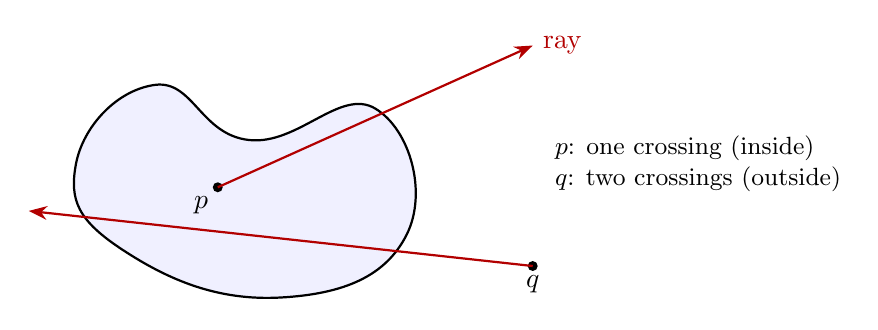
\begin{tikzpicture}[scale=1]
  \draw[thick,fill=blue!6] plot[smooth cycle,tension=0.8] coordinates {(0,0) (2,-0.6) (3.6,0.2) (3.2,1.8) (1.6,1.4) (0.4,2.1) (-0.6,1.1)};
  \fill (1.2,0.8) circle (1.8pt) node[below left] {$p$};
  \draw[-{Stealth},red!70!black,thick] (1.2,0.8) -- (5.2,2.6) node[right] {ray};
  \fill (5.2,-0.2) circle (1.8pt) node[below] {$q$};
  \draw[-{Stealth},red!70!black,thick] (5.2,-0.2) -- (-1.2,0.5);

  \node[font=\small,align=left] at (7.3,1.1) {$p$: one crossing (inside)\\ $q$: two crossings (outside)};
\end{tikzpicture}
\caption{Point-in-object by ray casting: an odd number of crossings means inside.}
\label{fig:raycast}
\end{figure}

For many points against one body, a caller-held query builds the LBVH once:
\begin{lstlisting}[numbers=none]
MFTL_PointQuery *MFTLPointQueryCreate(MFTL_Object *obj);          /* collective */
int  MFTLPointQueryInside(MFTL_PointQuery *q, const double p[3]);
int  MFTLPointQueryInsideMany(MFTL_PointQuery *q, int n, const double *xyz, int *result);
void MFTLPointQueryDestroy(MFTL_PointQuery **q);
\end{lstlisting}
\fn{MFTLPointQueryInsideMany} classifies $n$ points (the same points on every rank) with the same
ray sequence and verdicts as $n$ single calls, but with $O(\text{retries})$ collectives instead of
$O(n)$. The query stays valid until the body changes. \textbf{Known defect:} on a non-periodic
domain the caller-held query deadlocks when some rank stores no triangle of the body; use it
only when every rank holds part of the body, as the example of \S\ref{sec:ex-queries} does
(\S\ref{sec:known-defects}).

\fn{MFTLPointTriangleDistance}\texttt{(obj, t, p)} returns the exact distance from a point to a
stored triangle (the \mftlone{} six-region classification); it uses the stored positions as
given, without minimum image, and is rank-local.

\section{The linear bounding-volume hierarchy}

\fn{MFTL\_GenerateLBVH}\texttt{(obj)} builds a bounding-volume hierarchy over all stored triangles
of an object (rank-local):
\begin{enumerate}
  \item the triangle centroids are normalised to their bounding box, quantised to $2^{10}$ cells
    per axis and interleaved into 30-bit Morton codes (Z-order);
  \item the (code, index) pairs are sorted with a radix sort;
  \item the tree is built top-down by splitting a range where the highest bit in which the keys
    of its first and last element differ changes; leaves hold at most four triangles;
  \item node boxes are refitted bottom-up, stored in single precision and inflated by
    $10^{-4}$.
\end{enumerate}
Nodes are 32 bytes (two per cache line). \fn{MFTL\_DestroyBVH} frees the tree.

\section{Triangle intersection}
\label{sec:intersection}

\fn{MFTL\_IntersectObjects}\texttt{(A, bvhA, B, bvhB, callback, user)} traverses two hierarchies
simultaneously and calls
\begin{lstlisting}[numbers=none]
typedef void (*IntersectionCallback)(MFTL_Object *objA, int triA, MFTL_Object *objB, int triB,
                                     void *user_data);
\end{lstlisting}
for every pair of stored triangles that intersect or come within $10^{-6}$ of each other. The
pair test is the Guigue--Devillers triangle test built on orientation predicates
(\fn{MFTL\_TriTriIntersect}), extended with nine edge--edge and six vertex--face distances for
the proximity. On a periodic domain the box tests shift by one period and each tested pair is
first placed in one common frame. Exactly coplanar pairs are reported as intersecting.

\fn{MFTLEnsembleIntersectObjects}\texttt{(ensA, ensB, callback, user)} is the collective driver:
it creates pairwise spatial ghosts, builds one LBVH per object and traverses every object pair
(pairs $i<j$ of one ensemble when \texttt{ensB} is \texttt{NULL}). The callback runs rank-locally
on stored triangles, so a pair near a rank boundary may be reported on two ranks.

\section{Overlap volumes}

\fn{MFTLEnsembleCalculateOverlap}\texttt{(ensA, ensB, \&records, \&n)} quantifies how much bodies
overlap, triangle pair by triangle pair (the \mftlone{} algorithm, with four documented
corrections). For each candidate pair the two triangles are projected on the plane normal to the
separation of the two bodies, the projected triangles are clipped against each other, and the
prism between the two sheets over the clip polygon gives a volume
$\tfrac13 A\sum(h_A-h_B)$ with exact zero crossings. Each record (\texttt{MFTL\_Overlap}) holds the
volume, the overlap areas on both sheets, the average surface normal
$\tfrac12(\vect{n}_A-\vect{n}_B)$, the centre of the overlap volume, an effective radius of
curvature and the global ids of the pair. The candidates are gathered with an all-gather
(owned triangles whose box meets the other body's box), every record is computed once, and the
full, deterministically ordered list is returned on every rank. On a periodic domain every body
must be compact and lie within half a period of its surface centre. \fn{MFTLCalculateOverlap}
computes a single pair. The 2-D helpers \fn{MFTLConvexHull2D}, \fn{MFTLPolygonArea2D} and
\fn{MFTLPolygonCentroid2D} are public as well.

\chapter{Remeshing}
\label{ch:remeshing}

A front-tracking surface is stretched and compressed by the flow; without intervention its
triangles degenerate. Remeshing keeps edge lengths within a window around a target length by
three local operators --- split, collapse and flip --- followed by tangential smoothing, and
optionally restores the enclosed volume that the operators change slightly.

\section{Parameters}

All parameters are in one structure, initialised completely by
\begin{lstlisting}[numbers=none]
void MFTLInitRemeshParams(MFTL_RemeshParameters *params, MFTL_RemeshType type, double target_length,
                          int iterations, MFTL_SmoothMode smooth_mode,
                          double feature_angle_threshold);
\end{lstlisting}
With \texttt{MFTL\_REMESH\_ISOTROPIC} the edge-length window is the Botsch--Kobbelt window
$[\tfrac45 h,\tfrac43 h]$ around the target length $h$. The defaults follow \mftlone: the
Botsch--Kobbelt criterion, the paraboloid vertex fit, quality gates, no volume-conserving
smoothing, load balancing and boundary cleanup on. Important fields:
\begin{description}
  \item[\texttt{criterion}] \texttt{MFTL\_CRITERION\_BOTSCH\_KOBBELT} (edge length),
    \texttt{\_BOTSCH\_KOBBELT\_CURVATURE} (curvature-adaptive length),
    \texttt{\_TRIANGLE\_AREA}, \texttt{\_JIAO};
  \item[\texttt{vertex\_fit}] where a new or moved vertex is placed: \texttt{MFTL\_FIT\_PARABOLOID}
    (least-squares paraboloid through the neighbourhood, LAPACK \texttt{dgelsy}; without LAPACK or
    for a rank-deficient fit the barycentric fit), \texttt{MFTL\_FIT\_BARYCENTRIC},
    \texttt{MFTL\_FIT\_NONE} (the midpoint);
  \item[\texttt{smooth\_mode}, \texttt{max\_smoothing\_iter}] tangential smoothing (vertex- or
    triangle-based centroid, quality-driven, curvature-based);
  \item[\texttt{volume\_conserving\_smoothing}] \texttt{MFTL\_VCSMOOTH\_KUPRAT} or
    \texttt{\_TSUR} after the pass;
  \item[\texttt{load\_balance}, \texttt{boundary\_cleanup}] the parallel driver
    (\S\ref{sec:parallel-remesh});
  \item[\texttt{skip\_*}, \texttt{fixed\_iterations}, \texttt{quiet}, \texttt{mftl1\_criteria}]
    \mftlone-parity switches, all off by default; \multi's front tracking sets them to reproduce
    \mftlone's remeshing;
  \item[\texttt{boundary\_corner\_angle}] the corner threshold of the generalized remesher
    (default $30^\circ$);
  \item[\texttt{stat\_splits}, \texttt{stat\_collapses}, \texttt{stat\_flips},
    \texttt{stat\_recovery\_skipped}] outputs, accumulated by every driver call.
\end{description}

\section{Operators}

\begin{figure}[ht]
\centering
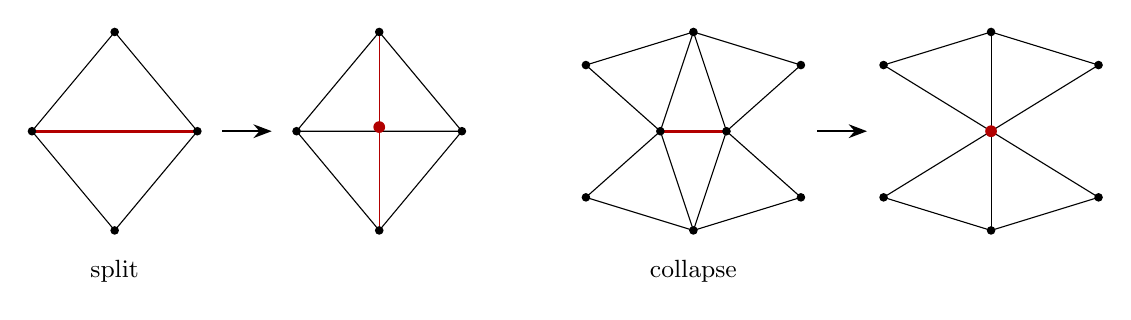
\begin{tikzpicture}[scale=1.05,v/.style={circle,fill=black,inner sep=1.1pt},n/.style={circle,fill=red!70!black,inner sep=1.5pt}]
  % split
  \begin{scope}
    \coordinate (a) at (0,0); \coordinate (b) at (2,0); \coordinate (c) at (1,1.2); \coordinate (d) at (1,-1.2);
    \draw (a)--(b)--(c)--cycle; \draw (a)--(d)--(b);
    \draw[very thick,red!70!black] (a)--(b);
    \foreach \p in {a,b,c,d} \node[v] at (\p) {};
    \node[font=\small] at (1,-1.7) {split};
    \draw[-{Stealth},thick] (2.3,0) -- (2.9,0);
    \begin{scope}[xshift=3.2cm]
      \coordinate (a) at (0,0); \coordinate (b) at (2,0); \coordinate (c) at (1,1.2); \coordinate (d) at (1,-1.2); \coordinate (m) at (1,0.05);
      \draw (a)--(b)--(c)--cycle; \draw (a)--(d)--(b); \draw[red!70!black] (c)--(m)--(d);
      \foreach \p in {a,b,c,d} \node[v] at (\p) {}; \node[n] at (m) {};
    \end{scope}
  \end{scope}
  % collapse
  \begin{scope}[xshift=7cm]
    \coordinate (a) at (0.6,0); \coordinate (b) at (1.4,0); \coordinate (c) at (1,1.2); \coordinate (d) at (1,-1.2);
    \coordinate (e) at (-0.3,0.8); \coordinate (f) at (-0.3,-0.8); \coordinate (g) at (2.3,0.8); \coordinate (h) at (2.3,-0.8);
    \draw (a)--(b)--(c)--cycle; \draw (a)--(d)--(b); \draw (e)--(a)--(f); \draw (e)--(c); \draw (f)--(d); \draw (g)--(b)--(h); \draw (g)--(c); \draw (h)--(d);
    \draw[very thick,red!70!black] (a)--(b);
    \foreach \p in {a,b,c,d,e,f,g,h} \node[v] at (\p) {};
    \node[font=\small] at (1,-1.7) {collapse};
    \draw[-{Stealth},thick] (2.5,0) -- (3.1,0);
    \begin{scope}[xshift=3.6cm]
      \coordinate (m) at (1,0); \coordinate (c) at (1,1.2); \coordinate (d) at (1,-1.2);
      \coordinate (e) at (-0.3,0.8); \coordinate (f) at (-0.3,-0.8); \coordinate (g) at (2.3,0.8); \coordinate (h) at (2.3,-0.8);
      \draw (e)--(m)--(f); \draw (g)--(m)--(h); \draw (c)--(m)--(d); \draw (e)--(c)--(g); \draw (f)--(d)--(h);
      \foreach \p in {c,d,e,f,g,h} \node[v] at (\p) {}; \node[n] at (m) {};
    \end{scope}
  \end{scope}
\end{tikzpicture}\\[2ex]
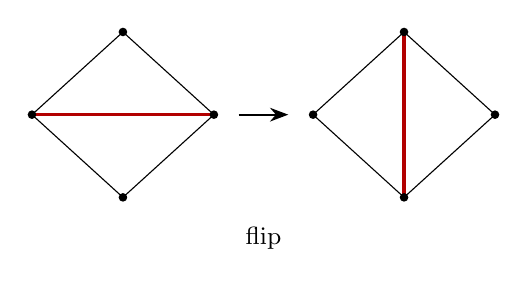
\begin{tikzpicture}[scale=1.05,v/.style={circle,fill=black,inner sep=1.1pt}]
  \coordinate (a) at (0,0); \coordinate (b) at (2.2,0); \coordinate (c) at (1.1,1.0); \coordinate (d) at (1.1,-1.0);
  \draw (a)--(c)--(b)--(d)--cycle; \draw[very thick,red!70!black] (a)--(b);
  \foreach \p in {a,b,c,d} \node[v] at (\p) {};
  \draw[-{Stealth},thick] (2.5,0) -- (3.1,0);
  \begin{scope}[xshift=3.4cm]
    \coordinate (a) at (0,0); \coordinate (b) at (2.2,0); \coordinate (c) at (1.1,1.0); \coordinate (d) at (1.1,-1.0);
    \draw (a)--(c)--(b)--(d)--cycle; \draw[very thick,red!70!black] (c)--(d);
    \foreach \p in {a,b,c,d} \node[v] at (\p) {};
  \end{scope}
  \node[font=\small] at (2.8,-1.5) {flip};
\end{tikzpicture}
\caption{The three topological operators. Split inserts a vertex on a long edge and splits both
adjacent triangles; collapse merges the two ends of a short edge into one vertex (removing two
triangles); flip replaces the diagonal of two triangles.}
\label{fig:operators}
\end{figure}

The operators (\texttt{mftl\_remeshing.h}) act rank-locally on stored entities
(Figure~\ref{fig:operators}):
\begin{description}
  \item[\fn{MFTLSplitEdge}] splits an edge at its midpoint (an interior or a boundary edge,
    never a REMOTE one) and returns the new vertex; the new vertex is placed by the displacement
    rule (\S\ref{sec:displacement}). \fn{MFTLSplitEdgeWithFit} then moves it onto the fitted
    surface.
  \item[\fn{MFTLCollapseEdge}] collapses $a\to b$; the survivor moves to the midpoint (or the
    fitted point with \fn{MFTLCollapseEdgeWithFit}).
  \item[\fn{MFTLFlipEdge}] flips an interior edge in place.
\end{description}
Removed entities are flagged \texttt{MFTL\_FLAG\_DEAD} during a pass;
\fn{MFTLFinalizeRemeshing} compacts the arrays afterwards (before any redistribution). The
approval gates \fn{MFTLSplitApproved}, \fn{CollapseApproved} and \fn{FlipApprovedWithParams}
apply the criterion, the link condition, quality and dihedral-angle gates, and the protection
of sharp features (\fn{MFTLDetectFeatures} flags edges whose dihedral angle exceeds the feature
angle). The operators keep the twin states: splits create LOCAL pairs and a boundary split
gives both halves the parent's tag; a collapse merges the states of the two outer
half-edges and is refused if one of them is REMOTE.

\paragraph{Criteria.} The Botsch--Kobbelt criterion splits edges longer than
\texttt{max\_edge\_length} and collapses edges shorter than \texttt{min\_edge\_length}. Its
curvature variant replaces the fixed target by the edge length that keeps the deviation from
the surface below $\varepsilon$ (\fn{MFTLBotschKobbeltCurvatureThreshold}): with
$\kappa_{\max}=\bar H+\sqrt{\bar H^2-\bar K}$ per endpoint, $\bar H$ and $\bar K$ being the stored
mean and Gaussian curvatures (Chapter~\ref{ch:geometry}),
\begin{equation}
  L = \sqrt{6\varepsilon/\kappa_{\max}-3\varepsilon^2},
\end{equation}
clamped to the window; the edge is split above $\tfrac43L$ and collapsed below $0.8L$. The
triangle quality used by the gates is the \mftlone{} measure
$q=(\text{perimeter}^2/A)/20.78460969$ (1 for an equilateral triangle, larger is worse;
\fn{MFTL\_TriangleQuality}).

\section{Smoothing and volume conservation}
\label{sec:volume-recovery}

\fn{MFTLSmoothTangential} (and \fn{MFTLSmoothTangentialWithParams}) move interior vertices in
their tangent plane towards the centroid of their neighbours or fan; vertices on a feature line
move along it; corners and boundary or rim vertices stay fixed. Two volume-conserving smoothers
are available: Kuprat's volume-conserving Laplacian (\fn{MFTLVolumeConservingSmoothing}, per edge
an exact first-order volume correction) and Jiao's TSUR3D null-space smoothing
(\fn{MFTLTSUR3D}); \fn{MFTLRoughnessSmoothing} applies them where the roughness exceeds its
thresholds. The serial versions refuse to run on a distributed mesh; the \texttt{...Parallel}
versions gate every edge to ``both endpoints owned, complete local fan''.

\paragraph{Volume recovery} (\fn{MFTLVolumeRecovery}\texttt{(obj, V\_target)}, collective) moves every
owned vertex along its normal by
\begin{equation}
  h = \frac{V-V_{\text{target}}}{A_{\text{eff}}}
\end{equation}
where $A_{\text{eff}}$ weights each owned triangle by the fraction of its corners owned by the rank
(exact first order in parallel); after the first step the slope is replaced by the measured
secant. It iterates until the relative error is below $10^{-12}$ (at most 10 steps; the stop
decision is reduced over ranks) and returns the final relative error. For a body that does not
enclose a volume by itself (open or wrapping) it does nothing and returns 0; use
\fn{MFTLPhaseSetVolumeRecovery} for sets.

\section{Surfaces with boundary: the generalized remesher}

Open bodies --- and closed bodies opted in with
\fn{MFTLObjectSetRemeshMode}\texttt{(obj, MFTL\_REMESH\_MODE\_GENERALIZED)} --- are remeshed by the
generalized, boundary-aware remesher. Closed bodies in the default mode use the closed-surface
remesher (with \texttt{mftl1\_criteria} set: bit-for-bit the \mftlone{} criteria). The selection
depends only on the declared class and the explicit mode, never on periodicity or on a body
touching a seam.

\paragraph{Link condition.} A collapse must not change the topology. The generalized remesher
uses the link condition on the complex augmented by one virtual vertex $\omega$ joined to every
boundary vertex (a virtual triangle $(u,v,\omega)$ per boundary edge): the collapse of $ab$ is
legal iff $\operatorname{Lk}(a)\cap\operatorname{Lk}(b)=\operatorname{Lk}(ab)$ in the augmented
complex. This single test forbids pinching a narrow strip, merging two boundary loops, creating
bow-ties, closing small holes and letting components vanish, while allowing the collapse of an
``ear'' triangle at the boundary.

\paragraph{Boundary curves and corners.} Every boundary tag has a boundary-curve mode
(\fn{MFTLObjectSetBoundaryCurve}):
\begin{itemize}
  \item \texttt{MFTL\_BCURVE\_REPRESENTED} (default): the curve is the interpolating Catmull--Rom
    spline through the loop's vertices; new boundary vertices are placed on it, so repeated
    remeshing does not shrink the loop;
  \item \texttt{MFTL\_BCURVE\_CONSTRAINED}: new and moved boundary vertices are projected by an
    application callback \texttt{MFTL\_BoundaryProjector} (a wall line, a ring, a support);
    \texttt{freeze} keeps the boundary vertices of the tag fixed during smoothing (used for
    pinned boundaries).
\end{itemize}
A boundary vertex whose turning angle exceeds the corner angle, or that carries
\texttt{MFTL\_VFLAG\_CORNER}, is a corner: it is never moved, merged or collapsed.

\paragraph{Other rules.} Boundary edges are never flipped; flips next to the boundary aim at
valence 6 inside, 4 on a straight boundary and $\operatorname{round}(\theta/60^\circ)+1$ at a
boundary vertex with interior angle $\theta$. Boundary vertices move only along their boundary
curve during smoothing. The volume-conserving smoothers act only on edges whose endpoints both
have closed fans.

\paragraph{Class-guarded volume recovery.} The drivers recover a body's volume only when it is
defined: its own volume for a closed compact body, the volume of its singleton phase set when
that is \texttt{MFTL\_DEFINED}, and nothing otherwise (counted in
\texttt{stat\_recovery\_skipped}).

\section{Drivers}
\label{sec:serial-bracket}

\paragraph{Serial.} \fn{MFTLRemeshEnsemble}\texttt{(ens, params)} runs the split, collapse, flip and
smoothing passes on every object, compacts, applies the optional volume-conserving smoothing and
the class-guarded volume recovery. Its edge kernel is rank-local, so on a distributed ensemble it
is run inside a \emph{serial bracket}:
\begin{lstlisting}[numbers=none]
MFTL_SerialBracket br;
MFTLEnsembleBeginSerial(ens, &br);      /* gather every object on rank 0 */
MFTLRemeshEnsemble(ens, &params);
MFTLEnsembleEndSerial(ens, &br, 1);     /* restore the decomposition and redistribute */
\end{lstlisting}
The bracket is also the way to run any serial kernel (TSUR3D, restart output) on a distributed
ensemble.

\paragraph{Parallel.}
\label{sec:parallel-remesh}
\fn{MFTLRemeshEnsembleParallel}\texttt{(ens, params)} (collective) chooses the algorithm:
\begin{itemize}
  \item on one rank, the serial kernel;
  \item for an ensemble of type \texttt{MFTL\_ENSEMBLE\_DISPERSED} whose largest body box is
    smaller than $0.5\,h_{\min}$ ($h_{\min}$: the smallest rank-box width), \emph{centering}:
    the ensemble is gathered on rank 0 and remeshed serially
    (\fn{MFTLRemeshEnsembleDispersedCentering});
  \item otherwise the \mftlone{} \emph{two-pass shift scheme}
    (\fn{MFTLRemeshEnsembleShiftScheme}).
\end{itemize}
The shift scheme (Figure~\ref{fig:shift}) first computes an x-only slab decomposition that
equalises the number of owned triangles per slab (\fn{MFTLRedistributeEnsembleLoadBalanced}); on a
decomposition that is not x-only, a temporary x-only layout is used and the native one restored
afterwards. Pass~1 remeshes on every rank the edges that are interior to it (both endpoints and
the complete fans owned); per-rank blocks of global ids are handed out before any split. Then
the cuts are shifted by $\max(0.2\,w_{\min},3\ell_{\text{ref}})$ ($w_{\min}$: the smallest slab
width, $\ell_{\text{ref}}$: \texttt{reference\_length}; \fn{MFTLShiftOwnershipRanges}) so that the
edges that straddled a cut become interior, and pass~2 remeshes them. Finally the few edges
that straddle both the old and the shifted cut are remeshed after gathering them on rank 0
(boundary cleanup), and a split cleanup pass follows. The mesh is returned redistributed on the
native decomposition, at a quiescent point.

\begin{figure}[ht]
\centering
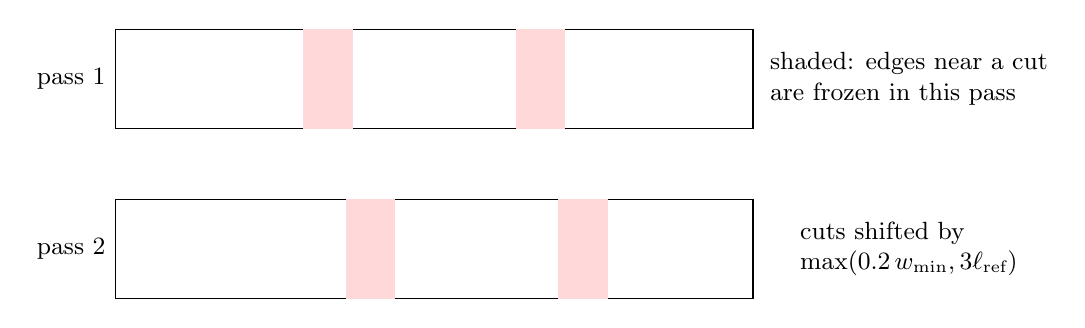
\begin{tikzpicture}[scale=0.9]
  \foreach \y/\lab/\sh in {2.4/pass 1/0, 0/pass 2/0.6} {
    \draw (0,\y) rectangle (9,\y+1.4);
    \foreach \x in {3,6} { \draw[very thick,dashed] (\x+\sh,\y) -- (\x+\sh,\y+1.4); }
    \foreach \x in {3,6} { \fill[red!15] (\x+\sh-0.35,\y) rectangle (\x+\sh+0.35,\y+1.4); }
    \node[left,font=\small] at (0,\y+0.7) {\lab};
  }
  \node[font=\small,align=left] at (11.2,3.1) {shaded: edges near a cut\\ are frozen in this pass};
  \node[font=\small,align=left] at (11.2,0.7) {cuts shifted by\\ $\max(0.2\,w_{\min},3\ell_{\text{ref}})$};
\end{tikzpicture}
\caption{The two-pass shift scheme on x-only slabs: edges near a cut are frozen in pass 1 and
remeshed in pass 2 after the cuts have been shifted.}
\label{fig:shift}
\end{figure}

\fn{MFTLRemeshEnsembleParallel} runs \texttt{MFTL\_ENSEMBLE\_SPANNING} ensembles (large interfaces)
always with the shift scheme. The example of \S\ref{sec:ex-remesh} runs a serial and a parallel
cycle.

\chapter{Per-triangle data}
\label{ch:data}

\section{The opaque payload}

An application can attach a fixed-size block of bytes to every triangle of an object --- in
\multi{}, for example, forces and scalar histories per front element. The library never looks
inside the block; it only moves it with the triangle.

\begin{lstlisting}[numbers=none]
int   MFTLInitializeObjectData(MFTL_Object *object, size_t data_size);   /* collective contract */
void *MFTLGetTriangleData(const MFTL_Object *obj, const MFTL_Triangle *tri);
void  MFTLSetTriangleData(MFTL_Object *obj, MFTL_Triangle *tri, const void *src);
int   MFTLScatterTriangleData(MFTL_Ensemble *ens, khash_t(object_map) *object_lookup);
\end{lstlisting}
The contract:
\begin{itemize}
  \item \texttt{data\_size} is set with \fn{MFTLInitializeObjectData}, with the \emph{same} value
    on every rank, before any redistribution. The function allocates a zeroed block for every
    existing triangle; triangles created later (remeshing, transport) get blocks as well.
    Re-initialising with a different size is refused.
  \item The block must be plain data without pointers: it is shipped as \texttt{MPI\_BYTE}, and a
    pointer is only meaningful on the rank that wrote it.
  \item Every transport path (redistribution, ghost layers, spatial ghosts, scatter) checks first
    that \texttt{data\_size} agrees on all ranks (\fn{MFTLCheckTriangleDataSizeConsistency}) and
    returns \texttt{MFTL\_ERROR} otherwise; a silent mismatch would corrupt the stream.
  \item Blocks travel byte-exactly with their triangle, in owned and ghost copies alike.
  \item Only the owner's block is authoritative. After changing owned blocks, refresh the ghosts
    with the collective \fn{MFTLScatterTriangleData}.
  \item \texttt{data\_size} $=0$ (the default) disables the payload; \fn{MFTLGetTriangleData}
    then returns \texttt{NULL}.
\end{itemize}
The blocks are freed with the object.

\section{The conserved surface scalar}

Every triangle carries \texttt{surface\_scalar}, a concentration per unit area (the \mftlone{}
scalar concentration). The library conserves its \emph{mass} $\sum_T c_T A_T$:
\begin{itemize}
  \item it travels with the triangle through every redistribution, ghost and pack operation and
    is written and read by the native mesh I/O;
  \item split, flip and collapse remap it mass-conservingly;
  \item the smoothing and volume-conserving vertex moves of the remesher rescale it by
    $A_{\text{old}}/A_{\text{new}}$;
  \item it starts at 0 for generated or built triangles.
\end{itemize}
Vertex moves made by the application do \emph{not} rescale it: an application that advects the
surface decides itself whether stretching dilutes the concentration. The example of
\S\ref{sec:ex-data} checks the byte-exact transport and the mass conservation.

\chapter{Interaction with multiflow}
\label{ch:multiflow}

\multi{} uses \mftl{} for its front-tracking interfaces and immersed-boundary bodies. This
chapter describes the interface between the two as it stands after Stage~16; the details live in
\multi{} (\texttt{src/general/mftlwrapper/}, \texttt{src/include/mftl\_adapter*.h} and
\texttt{src/interfacial/fronttracking/}).

\section{The adapter}

\multi{} never calls \mftl{} directly from its physics code. An adapter layer
(\texttt{mftl\_adapter.h}, implemented in \texttt{mftl\_adapter\_mftl2.c}) offers the operations
the solver needs --- body lists, iteration over triangles and vertices, positions, geometry in
local frames, redistribution, remeshing, I/O --- and maps them onto \mftl:
\begin{itemize}
  \item the decomposition of \multi's front-tracking overlap mesh (its particle-box grid)
    becomes the domain of an ensemble created with \fn{MFTLEnsembleCreateRectilinear}, with the
    per-axis cuts and the rank map of that grid. It is aligned with, but not identical to, the
    fluid partition; \multi's \texttt{sendnonlocal*} exchanges reconcile the two;
  \item per-body operations that \mftl{} implements for ensembles (remeshing, serial brackets)
    run on a one-object view of the body's ensemble;
  \item every redistribution first refreshes the cached centres of the owned triangles (the
    ownership rule of \S\ref{sec:triprops});
  \item physics code reads positions only through adapter accessors that return local-frame or
    continuous coordinates (\texttt{MFAdapterTriVertexPositions}, \texttt{MFAdapterVertContinuous},
    \texttt{MFAdapterVertDelta}, \texttt{MFAdapterEdgeVector}), so no physics routine subtracts
    wrapped positions itself; after advection \texttt{MFAdapterBodyWrapVertices} applies the
    displacement rule;
  \item checked queries (volume, centre, inside/outside) return
    \texttt{MFADAPTER\_DEFINED}, \texttt{\_UNDEFINED} or \texttt{\_UNSUPPORTED}, mirroring the
    phase-set statuses.
\end{itemize}
\multi{} finds \mftl{} with \texttt{find\_package(MFTL2)} (its CMake variable \texttt{MFTL2\_ROOT})
and needs a LAPACK-enabled build for its default vertex fit.

\section{Declaring periodic and open fronts}

The front-tracking options that concern \mftl{} (all in the \texttt{FRONTTRACKING} section of the
options file) are explicit declarations; nothing is inferred from the geometry:
\begin{center}\small
\begin{tabularx}{\textwidth}{@{}lX@{}}
\toprule
Option & Meaning \\
\midrule
\texttt{PeriodicFronts XZ} & the fronts are periodic along the listed axes (each must be periodic in the fluid) \\
\texttt{BodyMesh <body> <file.gts>} & read the body from a GTS file instead of generating a sphere \\
\texttt{OpenSurface <body> BoundaryFromMesh} & the body is open; every unmatched edge of its mesh is a boundary, tagged per loop \\
\texttt{RemeshMode <body> GENERALIZED|DEFAULT} & opt a closed body into the generalized remesher \\
\texttt{SurfaceScalarBC <body> <tag|ALL> NEUMANN q} & scalar flux $q$ per unit length (positive outward along $\vect{\nu}$) at the loops with that tag \\
\texttt{SurfaceScalarBC <body> <tag|ALL> DIRICHLET c} & prescribed concentration at the loops \\
\texttt{SurfaceTensionBoundary <body> <tag|ALL> PINNED STATIC} & the loops are pinned to a static support \\
\texttt{SurfaceTensionBoundary <body> <tag|ALL> REJECT} & (default) refuse surface tension on this open body \\
\texttt{PhaseSetMember <body> <+1|-1>} & the open body is a member of the dispersed-phase set with this sign \\
\texttt{WallClosure <X|Y|Z> <MIN|MAX>} & the dispersed-phase set is closed at this (non-periodic) fluid wall \\
\bottomrule
\end{tabularx}
\end{center}
\texttt{ROBIN} (scalar) and \texttt{CONTACT\_LINE} and IBM/DEM supports (surface tension) are
reserved and rejected.

\section{The capability check}

At initialisation --- and again after every class transition --- \multi{} classifies every front
body as \emph{closed} (non-periodic fronts), \emph{closed periodic compact}, \emph{closed periodic
wrapping} or \emph{open}, and checks it against every enabled module. A conflict stops the run with
a message that names the module and the body. The rules:
\begin{itemize}
  \item surface-only modules (Frenet-element surface tension, surface scalar transport) run on
    every closed class;
  \item modules that need an enclosed phase (indicator function, CSF, integral surface tension,
    marching cubes with breakup and coalescence, volume recovery, force computation, generic
    acceleration, normal-corrected advection, IRL reconstruction) need a closed non-periodic
    front, or a periodic front whose dispersed-phase set is \texttt{MFTL\_DEFINED};
  \item on periodic fronts some modules are not yet implemented (CSF, integral surface tension,
    surface viscosity, normal-corrected advection, generic acceleration, force computation,
    divergence-free interpolation, IRL reconstruction); the phase modules also reject wrapping
    fronts;
  \item an open body runs a module only with the declarations the module needs: scalar
    transport needs a scalar boundary condition for every boundary tag (zero flux is never
    assumed); Frenet surface tension needs \texttt{PINNED STATIC} on every tag; the indicator
    and volume recovery need membership in a wall-closed, \texttt{DEFINED} dispersed-phase set whose
    loops are all pinned; CSF and IRL additionally need a non-periodic front and a two-ring
    fit stencil; integral surface tension, marching cubes and surface viscosity are rejected.
\end{itemize}

\section{Boundary conditions on open bodies}
\label{sec:mf-bcs}

\mftl{} supplies only geometry for boundary edges: tag, length $L_e$, tangent $\vect{t}$, conormal
$\vect{\nu}$, midpoint and the triangle height $h_T=2A_T/L_e$
(\fn{MFTLBoundaryEdgeGeometry}, \fn{MFTLBoundaryEdgeCentroidDistance}). \multi{} builds its
boundary conditions from them.

\paragraph{Surface scalar.} The scalar lives at triangle centroids; the distance from the centroid
to a boundary edge along $\vect{\nu}$ is $\delta_e=h_T/3$.
\begin{itemize}
  \item \texttt{NEUMANN q}: the face value in the gradient reconstruction is
    $c_f=c_T-q\,\delta_e/D$, the diffusion right-hand side gets $-qL_e$, and the mass changes by
    $-\sum qL_e\Delta t$ (zero for $q=0$);
  \item \texttt{DIRICHLET c}: the face value is $c_D$, and the two-point flux
    $D L_e(c_D-c_T)/\delta_{\text{eff}}$ uses $\delta_{\text{eff}}=\max(\delta_e,0.1L_e)$ (a floor
    that bounds the coefficient on slivers; every use is counted).
\end{itemize}
The advective flux across a boundary edge is zero (a material boundary).

\paragraph{Pinned surface tension.} For constant $\sigma$ the element force of a triangle is
$\sum_{\text{edges}}\sigma L\vect{\nu}_e$; summed over an open surface the interior edges cancel,
leaving the line force at the boundary. With \texttt{PINNED STATIC} the boundary vertices are held
on their support (their loop is a frozen, constrained boundary curve), the element forces are
spread to the fluid unchanged, and the line force
\begin{equation}
  \vect{R} = -\sum_{\text{loop}} \sigma L_e\,\vect{\nu}_e
\end{equation}
is the reaction on the support, reported per step: the fluid force plus $\vect{R}$ is zero to
round-off. A free boundary line force is never applied implicitly.

\section{Periodic fronts}

With \texttt{PeriodicFronts} the \mftl{} domain is periodic on the declared axes with the fluid
period. Peskin spreading and interpolation use wrapped cell ranges, VTU output draws seam
triangles per image, logs report continuous centroids on compact axes (and ``undefined''
otherwise), and restarts use native mesh version~2. Closed bodies keep the \mftlone-parity remesher
whether periodic or not; open bodies always use the generalized remesher.

\chapter{Invariants and conventions}
\label{ch:invariants}

The table collects the invariants that hold at every quiescent point and the conventions the
library maintains. The test suite checks each of them; the Stage-16 fuzz test additionally
applies random jitter, remeshing and redistribution to a closed and an open body on 1, 2, 4 and 8
ranks and checks the topological invariants (twin states and ghost completion, exactly-once
ownership, boundary edges, loops and tags) after every step.

\begin{center}\small
\begin{longtable}{@{}p{0.27\textwidth}p{0.68\textwidth}@{}}
\toprule
Invariant & Statement \\
\midrule
\endhead
Manifold, orientable & every edge has one or two triangles; every vertex has one fan; the winding is consistent; bow-ties, non-manifold edges and M\"obius strips are rejected by the builders and never created by the operators \\
Declared class & only a body declared open has boundary half-edges; the class is identical on every rank \\
Twin states & every live half-edge is LOCAL, REMOTE or BOUNDARY; LOCAL pairs are symmetric; every REMOTE id names a live authoritative half-edge that names it back; a boundary edge has the same tag on every rank \\
Boundary / rim / seam & decided by topology, ownership and image counters only, never by coordinates (Table~\ref{tab:brs}) \\
Exactly-once ownership & every entity has exactly one owner; the owner's copy is authoritative; vertices are owned by position, triangles by cached centre \\
Ghost completion & G1: every edge of an owned triangle is LOCAL or BOUNDARY; G2: the fan of every owned vertex is stored \\
Image counters & $\vect{X}=\texttt{pos}+\texttt{img}\odot\vect{L}$ is the continuous coordinate; \texttt{pos} is wrapped; every update follows the displacement rule; the counters travel with the vertex \\
Edge restriction & every edge is shorter than half a period on every periodic axis \\
Wrap flags & after canonicalisation, \texttt{wrap}$_k$ holds iff some cycle winds along $k$; cut edges along a compact axis do not exist \\
Winding & closed bodies are wound outward: outward normals and $V>0$ \\
Volume & $V=\frac16\sum\vect{x}_1\cdot(\vect{x}_2\times\vect{x}_3)$ over owned triangles, in continuous coordinates, for closed compact bodies; otherwise through a phase-boundary set \\
Surface centre, inertia & area-weighted vertex sum over $3A$; lumped-tetrahedron moment of inertia (\mftlone{} parity) \\
Curvature & mean curvature $2/R$ and Gaussian curvature $2/R^2$ on a sphere; boundary vertices flagged \texttt{CURV\_UNDEFINED} \\
Closed-phase quantities & returned only with status \texttt{MFTL\_DEFINED}; UNDEFINED and UNSUPPORTED carry no value \\
Boundary loops & identical on every rank, independent of the rank count and of seams; tags persist through remeshing \\
Rank independence & collective results agree on all ranks and (to round-off) across rank counts \\
Opaque data & flat plain data of \texttt{data\_size} bytes, identical size on all ranks, transported byte-exactly \\
Surface scalar & its mass $\sum c_TA_T$ is conserved by transport and by the remesher \\
Tolerances & fixed absolute guards \texttt{MFTL\_VERYSMALL} $=10^{-12}$ and \texttt{MFTL\_VERYVERYSMALL} $=10^{-15}$; scale-dependent decisions use mesh-relative tolerances in their modules; overlap uses \texttt{MFTL\_REL\_TOLERANCE} $=5\times10^{-7}$ \\
\bottomrule
\end{longtable}
\end{center}

\chapter{Worked examples}
\label{ch:examples}

The programs in this chapter are the files \texttt{examples/manual\_*.c}. They are built with the
library (\texttt{BUILD\_EXAMPLES}) and run by the test suite on 1, 2, 4 and 8 ranks
(\texttt{Manual-<program>-np<N>}); each returns a non-zero exit code when a check fails. Run them with,
for example, \texttt{mpirun -np 4 ./manual\_basic\_workflow}.

\section{A complete program: ensemble, body, redistribution, integrals}
\label{sec:ex-basic}

This program creates an ensemble on an x-only decomposition, generates a sphere, writes it to a
GTS file and reads it back into a second object, redistributes both, computes volume, surface
centre and moment of inertia, and moves the sphere with the recommended sequence of
\S\ref{ch:parallel}.

\lstinputlisting{../examples/manual_basic_workflow.c}

\section{Curvature and normals}
\label{sec:ex-curvature}

\lstinputlisting{../examples/manual_curvature.c}

\section{Point queries and intersection}
\label{sec:ex-queries}

\lstinputlisting{../examples/manual_queries.c}

\section{Per-triangle data and the surface scalar}
\label{sec:ex-data}

\lstinputlisting{../examples/manual_triangle_data.c}

\section{Serial and parallel remeshing}
\label{sec:ex-remesh}

\lstinputlisting{../examples/manual_remeshing.c}

\section{A periodic body and image counters}
\label{sec:ex-periodic}

\lstinputlisting{../examples/manual_periodic.c}

\section{An open surface and its boundary loop}
\label{sec:ex-open}

\lstinputlisting{../examples/manual_open_surface.c}

\section{Phase-set queries}
\label{sec:ex-phaseset}

\lstinputlisting{../examples/manual_phase_set.c}

\chapter{Limitations and known compromises}
\label{ch:limitations}

\section{Intentionally unsupported}

The following are outside the scope of \mftl{} after Stage~16 and are rejected explicitly
rather than approximated:
\begin{itemize}
  \item contact-line dynamics (the loops of a wall-closed open surface must be pinned), and
    pinned supports that move with an IBM or DEM body;
  \item free liquid-interface edges, surface viscosity and integral surface tension on open
    surfaces, and mass properties derived from open surfaces;
  \item phase-set quantities whose status is UNDEFINED or UNSUPPORTED (Chapter~\ref{ch:phasesets});
  \item non-manifold, non-orientable and self-intersecting meshes (embeddedness is assumed, not
    checked);
  \item the \mftlone{} criteria (\texttt{mftl1\_criteria}) on open bodies.
\end{itemize}

\section{Performance compromises}

These are correct but not optimal; they are candidates for a later performance stage:
\begin{itemize}
  \item load balancing for parallel remeshing is one-dimensional (x-only slabs); on other
    decompositions a temporary x-only layout is used;
  \item the boundary cleanup of the parallel remesher, the centering algorithm and the serial
    bracket gather data on rank 0;
  \item canonicalisation gathers the edge graph of a body on rank 0; boundary loops and
    phase-set evaluations gather their records on every rank; the overlap driver all-gathers its
    candidates;
  \item \fn{MFTLPointInsideObject} builds an LBVH per call (use the caller-held query for many
    points); on periodic domains the caller-held query falls back to single-point calls;
  \item every triangle's payload is a separate heap block;
  \item \fn{MFTLUpdateGhostPositions} and \fn{MFTLScatterTriangleData} look up bodies linearly
    unless the caller passes a body-id map;
  \item spatial search over wrapping bodies uses conservative, stretched boxes for triangles that
    cross a seam.
\end{itemize}

\section{Behavioural limitations}

\begin{itemize}
  \item \fn{MFTLEnsembleCreateSpatialGhosts} compares boxes on the stored positions and is not
    periodic-aware (\fn{MFTL\_CreateSpatialGhosts}, used by the intersection driver, is).
  \item \fn{MFTLPointTriangleDistance} uses the stored positions without minimum image.
  \item The LBVH box inflation ($10^{-4}$) and the intersection proximity tolerance ($10^{-6}$)
    are absolute, not scaled with the mesh; exactly coplanar triangle pairs are reported as
    intersecting.
  \item \texttt{n\_local\_*} are maintained only by multi-rank redistributions, the builders,
    \fn{MFTLObjectAppendTriangleCopy} and \fn{MFTLObjectClear} (Chapter~\ref{ch:datamodel}).
  \item \fn{MFTLSwapEdge} is declared but not implemented; use \fn{MFTLFlipEdge}.
  \item The closed-surface parity collapse test checks the vertex part of the link condition
    only. For closed manifold meshes this cannot cause an illegal collapse (the only violating
    configuration is a tetrahedral component whose valence-3 vertices the \mftlone{} valence
    test already rejects); open bodies never use this path.
\end{itemize}

\section{Known defects}
\label{sec:known-defects}

Two defects were found during Stage~17. Fixing them changes behaviour, which Stage~17 (a
behaviour-preserving cleanup) does not do; they are recorded here for a later stage.
\begin{enumerate}
  \item \textbf{\fn{MFTLPointQueryInsideMany} / \fn{MFTLPointQueryInside} can deadlock.} On a
    non-periodic domain, a rank that stores no triangle of the body has no LBVH and takes the
    single-point fallback, while the other ranks run the batched loop; their collectives do not
    match. Work-around: use the caller-held query only when every rank stores at least one triangle
    of the body, or use \fn{MFTLPointInsideObject}. (\multi's adapter uses the caller-held query.)
  \item \textbf{Error path of \fn{MFTLEnsembleCreate}.} When the cuts do not match the number of
    ranks, or the communicators cannot be built, the partly initialised ensemble is destroyed
    with \fn{MFTLEnsembleDestroy}, which frees communicator handles that were never created and
    decrements the ensemble count that was never incremented (which can free the MPI datatypes
    while another ensemble is alive). Only the failure path is affected.
\end{enumerate}

\appendix
\chapter{Public API index}
\label{app:api}
\raggedright

The functions declared in the public headers, by header. Each name is declared in
\texttt{include/}; the documentation comment above the declaration states whether the function is
collective and what it requires. This list is generated from the headers.

\section*{\texttt{mftl\_core.h}}
\textit{Types:} \texttt{MFTL\_BoundaryCurve}, \texttt{MFTL\_Domain}, \texttt{MFTL\_Ensemble}, \texttt{MFTL\_HalfEdge}, \texttt{MFTL\_Object}, \texttt{MFTL\_Triangle}, \texttt{MFTL\_Vertex}\par
\textit{Functions:} \texttt{MFTLObjectCreate}, \texttt{MFTLGetTriangleData}, \texttt{MFTLSetTriangleData}, \texttt{MFTLInitializeObjectData}, \texttt{MFTLObjectDestroy}, \texttt{MFTLEnsembleUpdateGlobalCounts}, \texttt{MFTLObjectUpdateGlobalStats}, \texttt{MFTLEnsembleCreate}, \texttt{MFTLEnsembleCreateRectilinear}, \texttt{MFTLEnsembleSetDecomposition}, \texttt{MFTLEnsembleRemoveObject}, \texttt{MFTLDomainCreateTemporary}, \texttt{MFTLDomainFreeTemporary}, \texttt{MFTLEnsembleTransferObject}, \texttt{MFTLEnsembleAddObject}, \texttt{MFTLEnsembleDestroy}, \texttt{MFTLGenerateSphere}\par

\section*{\texttt{mftl\_constants.h}}
\textit{Types:} \texttt{MFTL\_EnsembleType}, \texttt{MFTL\_RemeshAlgorithm}\par

\section*{\texttt{mftl\_topology.h}}
\textit{Types:} \texttt{MFTL\_BoundaryDecl}, \texttt{MFTL\_BoundaryEdgeDecl}, \texttt{MFTL\_BoundaryLoop}, \texttt{MFTL\_BoundaryLoopSet}, \texttt{MFTL\_DiscoveryStats}, \texttt{MFTL\_Neighborhood}\par
\textit{Functions:} \texttt{MFTLGetVertex}, \texttt{MFTLGetHalfedge}, \texttt{MFTLGetTriangle}, \texttt{MFTLVOutHe}, \texttt{MFTLTHe}, \texttt{MFTLGetTriangleHalfedges}, \texttt{MFTLGetTriangleVertices}, \texttt{MFTLHeTarget}, \texttt{MFTLHeOrigin}, \texttt{MFTLHeTwin}, \texttt{MFTLHeIsLocal}, \texttt{MFTLHeIsRemote}, \texttt{MFTLHeIsBoundary}, \texttt{MFTLHeIsUnresolved}, \texttt{MFTLBoundaryCode}, \texttt{MFTLHeBoundaryTag}, \texttt{MFTLHeSetBoundary}, \texttt{MFTLHeSetRemote}, \texttt{MFTLHeTwinGid}, \texttt{MFTLHeTwinCode}, \texttt{MFTLHeEdgeId}, \texttt{MFTLHeNext}, \texttt{MFTLHePrev}, \texttt{MFTLHeTriangle}, \texttt{MFTLHeAdjacentTriangle}, \texttt{MFTLGetVertexOneRing}, \texttt{MFTLGetVertexOneRingVertices}, \texttt{MFTLGetVertexOneRingHalfedges}, \texttt{MFTLGetTriangleNeighbors}, \texttt{MFTLRebuildTwins}, \texttt{MFTLConvertGlobalToLocalIndices}, \texttt{MFTLFlattenConnectivity}, \texttt{MFTLCheckMeshIntegrity}, \texttt{MFTLFreeNeighborhood}, \texttt{MFTLGetNeighborhood}, \texttt{MFTLBuildTopologyFromTriples}, \texttt{MFTLBuildFromSoup}, \texttt{MFTLBuildFromSoupEx}, \texttt{MFTLBuildFromSoupImg}, \texttt{MFTLObjectAppendTriangleCopy}, \texttt{MFTLObjectCommitCopy}, \texttt{MFTLObjectDeclareOpen}, \texttt{MFTLVertexRing}, \texttt{MFTLCheckTwinStatesLocal}, \texttt{MFTLValidateTwinStatesEx}, \texttt{MFTLValidateTwinStates}, \texttt{MFTLCompleteGhosts}, \texttt{MFTLDiscoverySetForceFallback}, \texttt{MFTLGetLastDiscoveryStats}, \texttt{MFTLBoundaryLoops}, \texttt{MFTLFreeBoundaryLoops}, \texttt{MFTLRefreshBoundaryCache}, \texttt{MFTLObjectClear}\par

\section*{\texttt{mftl\_communication.h}}
\textit{Types:} \texttt{MFTL\_GidList}, \texttt{MFTL\_SendBuffer}\par
\textit{Functions:} \texttt{MFTLRegisterMpiTypes}, \texttt{MFTLFreeMpiTypes}, \texttt{MFTLSlabIndex}, \texttt{MFTLGetOwnerProc}, \texttt{MFTLRedistributeObject}, \texttt{MFTLRedistributeListOfObjects}, \texttt{MFTLRedistribute}, \texttt{MFTLPackSingleVertex}, \texttt{MFTLPackSingleTriangle}, \texttt{MFTLAppendGhostVertex}, \texttt{MFTLAppendGhostTriangle}, \texttt{MFTLCheckTriangleDataSizeConsistency}, \texttt{MFTLUpdateGhostPositions}, \texttt{MFTLScatterTriangleData}, \texttt{MFTLExtendGhostLayer}, \texttt{MFTLEnsembleCreateSpatialGhosts}, \texttt{MFTLObjectSendLocalTrianglesToAll}\par

\section*{\texttt{mftl\_geometry.h}}
\textit{Types:} \texttt{MFTL\_PointQuery}\par
\textit{Functions:} \texttt{MFTLGetMinimumImageVector}, \texttt{MFTLApplyPeriodicity}, \texttt{MFTLWrapPosImg}, \texttt{MFTLImgFollow}, \texttt{MFTLVertexRelative}, \texttt{MFTLEdgeShift}, \texttt{MFTLWrapContinuous}, \texttt{MFTLDomainAnyPeriodic}, \texttt{MFTLUnwrapToAnchor}, \texttt{MFTLGetEdgeLength}, \texttt{MFTL\_SQRT}, \texttt{MFTLGetEdgeLengthSquared}, \texttt{MFTLGetTriangleProperties}, \texttt{MFTLGetTriangleArea}, \texttt{MFTLGetTriangleNormal}, \texttt{MFTLGetTriangleCenter}, \texttt{MFTLComputeTriangleProperties}, \texttt{MFTLObjectVolume}, \texttt{MFTLSurfaceCenter}, \texttt{MFTLMomentOfInertia}, \texttt{MFTLCheckMinimumImageConstraint}, \texttt{MFTLVertexDelta}, \texttt{MFTLEdgeVector}, \texttt{MFTLVertexContinuous}, \texttt{MFTLTriangleUnwrapped}, \texttt{MFTLBoundaryEdgeGeometry}, \texttt{MFTLBoundaryEdgeCentroidDistance}, \texttt{MFTLVertexAngleSum}, \texttt{MFTLVertexTurningAngle}, \texttt{MFTLBoundaryNeighbours}, \texttt{MFTLFindThinRegionPairs}, \texttt{MFTLFindProximityPairs}, \texttt{MFTLScaleObject}, \texttt{MFTLTranslateObject}, \texttt{MFTLRotateObject}, \texttt{MFTLWrapObjectIntoDomain}, \texttt{MFTLGenerateCylinder}, \texttt{MFTLGenerateBox}, \texttt{MFTLGenerateCube}, \texttt{MFTLGenerateFace}, \texttt{MFTLComputeVertexNormals}, \texttt{MFTLComputeVertexCurvatures}, \texttt{MFTLComputeExtrapolatedCurvatures}, \texttt{MFTLComputeVertexNormalAt}, \texttt{MFTLComputeVertexCurvatureAt}, \texttt{MFTLComputeRoughness}, \texttt{MFTLPointTriangleDistance}, \texttt{MFTLPointInsideObject}, \texttt{MFTLPointQueryCreate}, \texttt{MFTLPointQueryDestroy}, \texttt{MFTLPointQueryInside}, \texttt{MFTLPointQueryInsideMany}, \texttt{MFTLPointInsideAABB}, \texttt{MFTLObjectAABB}, \texttt{MFTLDebugPointQueryBVHBuilds}, \texttt{MFTLDebugPointQueryLastIterations}\par

\section*{\texttt{mftl\_images.h}}
\textit{Functions:} \texttt{MFTLCanonicaliseImages}, \texttt{MFTLObjectRegaugeImages}, \texttt{MFTLObjectEnsureWinding}, \texttt{MFTLObjectWrapFlags}, \texttt{MFTLObjectIsCompact}, \texttt{MFTLObjectHasVolume}, \texttt{MFTLCheckWrapFlags}, \texttt{MFTLCountCutEdges}, \texttt{MFTLObjectReference}\par

\section*{\texttt{mftl\_phase\_set.h}}
\textit{Types:} \texttt{MFTL\_PhaseSet}, \texttt{MFTL\_PhaseSetInfo}, \texttt{MFTL\_PhaseSetTolerances}, \texttt{MFTL\_PhaseStatus}\par
\textit{Functions:} \texttt{MFTLPhaseSetCreate}, \texttt{MFTLPhaseSetDestroy}, \texttt{MFTLPhaseSetAddMember}, \texttt{MFTLPhaseSetAddWallClosure}, \texttt{MFTLPhaseSetClassify}, \texttt{MFTLPhaseSetVolume}, \texttt{MFTLPhaseSetCentre}, \texttt{MFTLPhaseSetInside}, \texttt{MFTLPhaseSetVolumeRecovery}, \texttt{MFTLPhaseSetGetTolerances}, \texttt{MFTLPhaseSetSetTolerances}\par

\section*{\texttt{mftl\_io.h}}
\textit{Functions:} \texttt{MFTLWriteVtk}, \texttt{MFTLWriteVtu}, \texttt{MFTLReadGTS}, \texttt{MFTLWriteGTS}, \texttt{MFTLWritePvtu}, \texttt{MFTLWriteNativeMesh}, \texttt{MFTLWriteNativeMeshV2}, \texttt{MFTLReadNativeMesh}\par

\section*{\texttt{mftl\_bvh.h}}
\textit{Types:} \texttt{MFTL\_BVH}, \texttt{MFTL\_BVHNode}\par
\textit{Functions:} \texttt{MFTL\_CreateSpatialGhosts}, \texttt{MFTL\_GenerateLBVH}, \texttt{MFTL\_DestroyBVH}, \texttt{MFTL\_IntersectObjects}, \texttt{MFTL\_TriTriIntersect}, \texttt{MFTLEnsembleIntersectObjects}\par

\section*{\texttt{mftl\_overlap.h}}
\textit{Types:} \texttt{MFTL\_Overlap}, \texttt{MFTL\_Point2D}\par
\textit{Functions:} \texttt{MFTLCalculateOverlap}, \texttt{MFTLEnsembleCalculateOverlap}, \texttt{MFTLConvexHull2D}, \texttt{MFTLPolygonArea2D}, \texttt{MFTLPolygonCentroid2D}\par

\section*{\texttt{mftl\_remeshing.h}}
\textit{Types:} \texttt{MFTL\_RemeshCriterion}, \texttt{MFTL\_RemeshOpType}, \texttt{MFTL\_RemeshParameters}, \texttt{MFTL\_RemeshType}, \texttt{MFTL\_SerialBracket}, \texttt{MFTL\_SmoothMode}, \texttt{MFTL\_VCSmoothMode}, \texttt{MFTL\_VertexFitMode}\par
\textit{Functions:} \texttt{MFTLInitRemeshParams}, \texttt{MFTLSplitEdge}, \texttt{MFTLCollapseEdge}, \texttt{MFTLSwapEdge}, \texttt{MFTLFlipEdge}, \texttt{FlipApprovedWithParams}, \texttt{MFTLFinalizeRemeshing}, \texttt{MFTL\_TriangleQuality}, \texttt{MFTLBotschKobbeltCurvatureThreshold}, \texttt{MFTLFitVertex}, \texttt{MFTLSplitEdgeWithFit}, \texttt{MFTLCollapseEdgeWithFit}, \texttt{MFTLSmoothTangentialWithParams}, \texttt{MFTLDetectFeatures}, \texttt{CollapseApproved}, \texttt{MFTLVolumeRecovery}, \texttt{MFTLEdgeVolumeConservingSmoothing}, \texttt{MFTLVolumeConservingSmoothing}, \texttt{MFTLEdgeTSUR}, \texttt{MFTLTSUR3D}, \texttt{MFTLRoughnessSmoothing}, \texttt{MFTLObjectSetRemeshMode}, \texttt{MFTLObjectRemeshGeneralized}, \texttt{MFTLObjectSetBoundaryCurve}, \texttt{MFTLObjectTakeClassTransition}, \texttt{MFTLRemeshEnsemble}, \texttt{MFTLSplitApproved}, \texttt{MFTL1SplitCriterion}, \texttt{MFTL1CollapseApproved}, \texttt{MFTL1FlipApproved}, \texttt{MFTL1Sweeps}, \texttt{MFTLRemeshEnsembleParallel}, \texttt{MFTLRemeshEnsembleShiftScheme}, \texttt{MFTLRemeshEnsembleDispersedCentering}, \texttt{MFTLEnsembleBeginSerial}, \texttt{MFTLEnsembleEndSerial}, \texttt{MFTLRedistributeEnsembleLoadBalanced}, \texttt{MFTLShiftOwnershipRanges}, \texttt{MFTLSyncEnsembleGidCounters}, \texttt{MFTLVolumeConservingSmoothingParallel}, \texttt{MFTLTSUR3DParallel}, \texttt{MFTLRoughnessSmoothingParallel}, \texttt{MFTLDomainGetHMin}\par

\section*{\texttt{mftl\_vectoroperations.h}}
\textit{Functions:} \texttt{MFTLNormalizeVector}, \texttt{MFTLVectorInProd}, \texttt{MFTLVectorCrossVector}\par

\section*{\texttt{mftl\_arrayfunctions.h}}
\textit{Functions:} \texttt{MFTLSortIds}, \texttt{MFTLSortPairs}, \texttt{MFTLRadixSort}, \texttt{MFTLGetUniqueIntegers}, \texttt{MFTLUniqueIntArray}, \texttt{MFTLUniquePairs}\par



\end{document}
